\PassOptionsToPackage{unicode=true}{hyperref} % options for packages loaded elsewhere
\PassOptionsToPackage{hyphens}{url}
%
\documentclass[]{book}
\usepackage{lmodern}
\usepackage{amssymb,amsmath}
\usepackage{ifxetex,ifluatex}
\usepackage{fixltx2e} % provides \textsubscript
\ifnum 0\ifxetex 1\fi\ifluatex 1\fi=0 % if pdftex
  \usepackage[T1]{fontenc}
  \usepackage[utf8]{inputenc}
  \usepackage{textcomp} % provides euro and other symbols
\else % if luatex or xelatex
  \usepackage{unicode-math}
  \defaultfontfeatures{Ligatures=TeX,Scale=MatchLowercase}
\fi
% use upquote if available, for straight quotes in verbatim environments
\IfFileExists{upquote.sty}{\usepackage{upquote}}{}
% use microtype if available
\IfFileExists{microtype.sty}{%
\usepackage[]{microtype}
\UseMicrotypeSet[protrusion]{basicmath} % disable protrusion for tt fonts
}{}
\IfFileExists{parskip.sty}{%
\usepackage{parskip}
}{% else
\setlength{\parindent}{0pt}
\setlength{\parskip}{6pt plus 2pt minus 1pt}
}
\usepackage{hyperref}
\hypersetup{
            pdftitle={Mini-Workshop Panel Data Analysis},
            pdfauthor={Marko Bachl (mit Material von Michael Scharkow)},
            pdfborder={0 0 0},
            breaklinks=true}
\urlstyle{same}  % don't use monospace font for urls
\usepackage{color}
\usepackage{fancyvrb}
\newcommand{\VerbBar}{|}
\newcommand{\VERB}{\Verb[commandchars=\\\{\}]}
\DefineVerbatimEnvironment{Highlighting}{Verbatim}{commandchars=\\\{\}}
% Add ',fontsize=\small' for more characters per line
\usepackage{framed}
\definecolor{shadecolor}{RGB}{248,248,248}
\newenvironment{Shaded}{\begin{snugshade}}{\end{snugshade}}
\newcommand{\AlertTok}[1]{\textcolor[rgb]{0.94,0.16,0.16}{#1}}
\newcommand{\AnnotationTok}[1]{\textcolor[rgb]{0.56,0.35,0.01}{\textbf{\textit{#1}}}}
\newcommand{\AttributeTok}[1]{\textcolor[rgb]{0.77,0.63,0.00}{#1}}
\newcommand{\BaseNTok}[1]{\textcolor[rgb]{0.00,0.00,0.81}{#1}}
\newcommand{\BuiltInTok}[1]{#1}
\newcommand{\CharTok}[1]{\textcolor[rgb]{0.31,0.60,0.02}{#1}}
\newcommand{\CommentTok}[1]{\textcolor[rgb]{0.56,0.35,0.01}{\textit{#1}}}
\newcommand{\CommentVarTok}[1]{\textcolor[rgb]{0.56,0.35,0.01}{\textbf{\textit{#1}}}}
\newcommand{\ConstantTok}[1]{\textcolor[rgb]{0.00,0.00,0.00}{#1}}
\newcommand{\ControlFlowTok}[1]{\textcolor[rgb]{0.13,0.29,0.53}{\textbf{#1}}}
\newcommand{\DataTypeTok}[1]{\textcolor[rgb]{0.13,0.29,0.53}{#1}}
\newcommand{\DecValTok}[1]{\textcolor[rgb]{0.00,0.00,0.81}{#1}}
\newcommand{\DocumentationTok}[1]{\textcolor[rgb]{0.56,0.35,0.01}{\textbf{\textit{#1}}}}
\newcommand{\ErrorTok}[1]{\textcolor[rgb]{0.64,0.00,0.00}{\textbf{#1}}}
\newcommand{\ExtensionTok}[1]{#1}
\newcommand{\FloatTok}[1]{\textcolor[rgb]{0.00,0.00,0.81}{#1}}
\newcommand{\FunctionTok}[1]{\textcolor[rgb]{0.00,0.00,0.00}{#1}}
\newcommand{\ImportTok}[1]{#1}
\newcommand{\InformationTok}[1]{\textcolor[rgb]{0.56,0.35,0.01}{\textbf{\textit{#1}}}}
\newcommand{\KeywordTok}[1]{\textcolor[rgb]{0.13,0.29,0.53}{\textbf{#1}}}
\newcommand{\NormalTok}[1]{#1}
\newcommand{\OperatorTok}[1]{\textcolor[rgb]{0.81,0.36,0.00}{\textbf{#1}}}
\newcommand{\OtherTok}[1]{\textcolor[rgb]{0.56,0.35,0.01}{#1}}
\newcommand{\PreprocessorTok}[1]{\textcolor[rgb]{0.56,0.35,0.01}{\textit{#1}}}
\newcommand{\RegionMarkerTok}[1]{#1}
\newcommand{\SpecialCharTok}[1]{\textcolor[rgb]{0.00,0.00,0.00}{#1}}
\newcommand{\SpecialStringTok}[1]{\textcolor[rgb]{0.31,0.60,0.02}{#1}}
\newcommand{\StringTok}[1]{\textcolor[rgb]{0.31,0.60,0.02}{#1}}
\newcommand{\VariableTok}[1]{\textcolor[rgb]{0.00,0.00,0.00}{#1}}
\newcommand{\VerbatimStringTok}[1]{\textcolor[rgb]{0.31,0.60,0.02}{#1}}
\newcommand{\WarningTok}[1]{\textcolor[rgb]{0.56,0.35,0.01}{\textbf{\textit{#1}}}}
\usepackage{longtable,booktabs}
% Fix footnotes in tables (requires footnote package)
\IfFileExists{footnote.sty}{\usepackage{footnote}\makesavenoteenv{longtable}}{}
\usepackage{graphicx,grffile}
\makeatletter
\def\maxwidth{\ifdim\Gin@nat@width>\linewidth\linewidth\else\Gin@nat@width\fi}
\def\maxheight{\ifdim\Gin@nat@height>\textheight\textheight\else\Gin@nat@height\fi}
\makeatother
% Scale images if necessary, so that they will not overflow the page
% margins by default, and it is still possible to overwrite the defaults
% using explicit options in \includegraphics[width, height, ...]{}
\setkeys{Gin}{width=\maxwidth,height=\maxheight,keepaspectratio}
\setlength{\emergencystretch}{3em}  % prevent overfull lines
\providecommand{\tightlist}{%
  \setlength{\itemsep}{0pt}\setlength{\parskip}{0pt}}
\setcounter{secnumdepth}{5}
% Redefines (sub)paragraphs to behave more like sections
\ifx\paragraph\undefined\else
\let\oldparagraph\paragraph
\renewcommand{\paragraph}[1]{\oldparagraph{#1}\mbox{}}
\fi
\ifx\subparagraph\undefined\else
\let\oldsubparagraph\subparagraph
\renewcommand{\subparagraph}[1]{\oldsubparagraph{#1}\mbox{}}
\fi

% set default figure placement to htbp
\makeatletter
\def\fps@figure{htbp}
\makeatother

\usepackage{booktabs}
\usepackage[]{natbib}
\bibliographystyle{apalike}

\title{Mini-Workshop Panel Data Analysis}
\author{Marko Bachl (mit Material von Michael Scharkow)}
\date{Sommersemester 2020 \textbar{} IJK Hannover}

\begin{document}
\maketitle

{
\setcounter{tocdepth}{1}
\tableofcontents
}
\hypertarget{uxfcberblick}{%
\chapter{Überblick}\label{uxfcberblick}}

\hypertarget{inhalt-des-virtuellen-mini-workshops}{%
\section{Inhalt des virtuellen Mini-Workshops}\label{inhalt-des-virtuellen-mini-workshops}}

\begin{itemize}
\item
  Der Mini-Workshop bietet eine \emph{pragmatische} Einführung in die Analyse von Panel-Daten aus Erhebungen mit mindestens drei Wellen. Konkret liegt der Fokus auf sogenannten \emph{micro panels}, also Datensätzen mit relativ vielen Fällen und relativ wenigen Messzeitpunkten (das klassische Befragungspanel).
\item
  In der Analyse beschränken uns hier auf Varianten der \emph{linearen} Regressionsmodelle. Wir beginnen mit den grundlegenden \emph{fixed effects} und \emph{random effects} Modellen. Dann betrachten wir das \emph{within-between} Modell, das als eine Integration des \emph{fixed effects} Modell in das \emph{random effects} Modell verstanden werden kann. Dies ist auch eine gute Grundlage für den Einstieg in verschiedene Erweiterungen, zum Beispiel zu verallgemeinerten linearen Modellen oder zu Wachstumskurvenmodellen. Diese sind aber nicht Teil dieses Mini-Workshops.
\item
  Wir schätzen die Modelle mit etablierten \emph{least-squares} und \emph{maximum likelihood} Methoden. Gerade bei den \emph{within-between} Modellen sind bayesianische Schätzmethoden, z.B. \emph{MCMC sampling} (implementiert in \href{https://mc-stan.org/}{Stan}), unabhängig von statistisch-philosophischen Überlegungen sehr interessant. Bei Interesse kann ich nur empfehlen, hier einen Einstieg zu finden.
\item
  Zur Aufbereitung der Daten, Visualisierung und Modell-Schätzung verwenden wir \texttt{R} mit dem \texttt{tidyverse} und eine kleine Zahl speziallisierter Pakete für die Modellschätzung. Der Fokus des Workshops liegt aber auf der substantiellen Arbeit mit den Modellen, nicht auf der Umsetzung in \texttt{R}.
\end{itemize}

\hypertarget{welche-inhalte-wir-nicht-behandeln}{%
\section{Welche Inhalte wir nicht behandeln}\label{welche-inhalte-wir-nicht-behandeln}}

\begin{itemize}
\item
  Der Workshop ist kein Statistik- oder Ökonometrie-Kurs. Ich bin --- wie auch ihr --- ausgebildeter Sozialwissenschaftler. Die statistischen Grundlagen, auf denen der Workshop aufbaut, gehen aus den Grundlagentexten \citep{bellExplainingFixedEffects2015, vaiseyWhatYouCan2017} hervor.
\item
  Grundkentnisse in \texttt{R} setze ich voraus, insbesondere Datentransformationen innerhalb des \texttt{tidyverse}. Wir werden aber keine komplizierten Dinge in \texttt{R} tun. Auch ohne weiterführende \texttt{R}-Kenntnisse sollten die Inhalte des Workshops in Bezug auf die datenanalystischen Verfahren klar werden.
\item
  Wir werden nicht viel Zeit auf die verschiedenen Schätzer, deren Effizienz und Bias, die verschiedenen Algorithmen und Datentransformationen verwenden.
\item
  Wir werden keine Beweise oder Ableitungen besprechen. Wir setzen keine Kenntnisse in Matrixalgebra voraus --- weder meiner- noch eurerseits.
\item
  Wir behandeln einen sehr kleinen Ausschnitt möglicher Modelle für Panel-Daten. Wir konzentrieren uns auf regressionsbasierte Modelle zur Schätzung kausaler Effekte. Damit behandeln wir insbesondere nicht die vielfälltigen Verfahren, die in einem SEM-Framework verortet sind: längsschnittliche Messmodelle, Prozessmodelle, (random intercept) cross-lagged panel Modelle, Latent State-Trait Modelle, etc. Auch Modelle, in denen die Zeit-Variable als kontinuierlich (z.B. Tag der Erhebung im Gegensatz zu Indikator für Panelwelle) verwendet wird (z.B. Continuous Time Structural Equation Modeling), behandeln wir nicht.
\item
  Fehlende Daten (Panelmortalität, Ausfall von Einheiten in einzelnen Wellen) sind ein großes Thema in der Längsschnittanalyse. Wir werden es hier ignorieren, bis auf den Hinweis, dass alle Fälle, die in mindestens zwei bzw. drei Wellen Daten haben, grundsätzlich Informationen zur Schätzung beitragen.
\end{itemize}

\hypertarget{aufbau-des-workshops}{%
\section{Aufbau des Workshops}\label{aufbau-des-workshops}}

\begin{itemize}
\tightlist
\item
  Inhaltlicher Aufbau: Siehe Kapitel-Gliederung
\end{itemize}

\hypertarget{material}{%
\subsection*{Material}\label{material}}
\addcontentsline{toc}{subsection}{Material}

\begin{itemize}
\item
  Dieses Dokument + R Skripte: (Hoffentlich) mehr oder weniger selbsterklärendes Material

  \begin{itemize}
  \tightlist
  \item
    Kuratierte Form ist dieses HTML-Dokument
  \item
    Es gibt auch ein PDF, das ich aber nicht formatiert habe
  \end{itemize}
\item
  Screencast: Ich gehe über das Material und erkläre es auf der Audio-Spur. Mal sehen, wie hilfreich das ist. Die Screencasts stelle ich über das LMS zur Verfügung.
\item
  Übungen: Zu einigen Analysen gibt es Übungsaufgaben.

  \begin{itemize}
  \tightlist
  \item
    Bei der \emph{Wiederholung} geht es darum, die Modelle leicht zu verändern (durch Anpassen der \texttt{R}-Skripte aus dem Material) und die Ergebnisse der angepassten Modelle zu interpretieren.
  \item
    Bei der \emph{Anwendung} geht es darum, in Anlehung an die Beispiele eigene Modelle zu spezifizieren und diese zu interpretieren.
  \end{itemize}
\end{itemize}

\hypertarget{pakete}{%
\subsection*{Pakete}\label{pakete}}
\addcontentsline{toc}{subsection}{Pakete}

Wir verwenden die folgenden Pakete

\begin{Shaded}
\begin{Highlighting}[]
\ControlFlowTok{if}\NormalTok{ (}\OperatorTok{!}\KeywordTok{require}\NormalTok{(}\StringTok{"pacman"}\NormalTok{)) }\KeywordTok{install.packages}\NormalTok{(}\StringTok{"pacman"}\NormalTok{)}
\NormalTok{pacman}\OperatorTok{::}\KeywordTok{p_load}\NormalTok{(tidyverse, ggstance, broom, broom.mixed, haven, plm, lmtest, lme4, }
\NormalTok{    performance)}
\KeywordTok{theme_set}\NormalTok{(}\KeywordTok{theme_bw}\NormalTok{())  }\CommentTok{# ggplot theme}

\KeywordTok{tibble}\NormalTok{(}\DataTypeTok{package =} \KeywordTok{c}\NormalTok{(}\StringTok{"R"}\NormalTok{, }\KeywordTok{sort}\NormalTok{(pacman}\OperatorTok{::}\KeywordTok{p_loaded}\NormalTok{()))) }\OperatorTok\StringTok{ }\KeywordTok{mutate}\NormalTok{(}\DataTypeTok{version =} \KeywordTok{map_chr}\NormalTok{(package, }
    \OperatorTok{~}\KeywordTok{as.character}\NormalTok{(pacman}\OperatorTok{::}\KeywordTok{p_version}\NormalTok{(}\DataTypeTok{package =}\NormalTok{ .x)))) }\OperatorTok\StringTok{ }\NormalTok{knitr}\OperatorTok{::}\KeywordTok{kable}\NormalTok{()}
\end{Highlighting}
\end{Shaded}

\begin{tabular}{l|l}
\hline
package & version\\
\hline
R & 3.6.2\\
\hline
broom & 0.5.4\\
\hline
broom.mixed & 0.2.4\\
\hline
dplyr & 0.8.4\\
\hline
forcats & 0.4.0\\
\hline
ggplot2 & 3.2.1\\
\hline
ggstance & 0.3.3\\
\hline
haven & 2.2.0\\
\hline
lme4 & 1.1.21\\
\hline
lmtest & 0.9.37\\
\hline
Matrix & 1.2.18\\
\hline
pacman & 0.5.1\\
\hline
performance & 0.4.6\\
\hline
plm & 2.2.3\\
\hline
purrr & 0.3.3\\
\hline
readr & 1.3.1\\
\hline
stringr & 1.4.0\\
\hline
tibble & 2.1.3\\
\hline
tidyr & 1.0.2\\
\hline
tidyverse & 1.3.0\\
\hline
zoo & 1.8.7\\
\hline
\end{tabular}

\hypertarget{einfuxfchrung}{%
\chapter{Einführung}\label{einfuxfchrung}}

\hypertarget{luxe4ngsschnittdaten}{%
\section{Längsschnittdaten}\label{luxe4ngsschnittdaten}}

\hypertarget{begriffe}{%
\subsection*{Begriffe}\label{begriffe}}
\addcontentsline{toc}{subsection}{Begriffe}

\begin{itemize}
\tightlist
\item
  Wiederholte Querschnittserhebungen (time series cross sectional, TSCS): \(n\) unabhängige Fälle (repräsentativ für dieselbe Grundgesamtheit) zu mehreren Messzeitpunkten \(t\).
\item
  Zeitreihe: Eine Einheit mit vielen Messzeitpunkten (\(n = 1\), \(t > 30\)).
\item
  Paneldaten: Dieselben Einheiten mit wiederholten Messungen (\(n > 30\), \(t \ge 2\))

  \begin{itemize}
  \tightlist
  \item
    Macro panel: \(n\) klein, \(t\) groß (z.B. jährliche Untersuchung von Staaten, 1950--2015)
  \item
    Micro panel: \(n\) groß, \(t\) klein (typisches Befragungspanel)
  \end{itemize}
\item
  In diesem Workshop geht es um \emph{micro panels} mit \(t > 2\)
\end{itemize}

\hypertarget{vorteile-von-paneldaten}{%
\subsection*{Vorteile von Paneldaten}\label{vorteile-von-paneldaten}}
\addcontentsline{toc}{subsection}{Vorteile von Paneldaten}

\begin{itemize}
\tightlist
\item
  Paneldaten erlauben die Identifikation von kausalen Effekten unter schwächeren Annahmen (im Vergleich zu Querschnittsdaten).

  \begin{itemize}
  \tightlist
  \item
    Wir haben einige (aber nicht perfekte!) Informationen über die zeitliche Abfolge von Veränderungen.
  \item
    Wir können untersuchen, ob, und wenn ja, wie ein Ereignis (eine Veränderung eines Prädiktors) das Kriterium verändert.
  \end{itemize}
\item
  Paneldaten erlauben die Untersuchung von individuellen Verläufen
\end{itemize}

\hypertarget{kausale-effekte-mit-paneldaten-schuxe4tzen}{%
\subsection*{Kausale Effekte mit Paneldaten schätzen}\label{kausale-effekte-mit-paneldaten-schuxe4tzen}}
\addcontentsline{toc}{subsection}{Kausale Effekte mit Paneldaten schätzen}

\hypertarget{bedingungen}{%
\subsubsection*{Bedingungen}\label{bedingungen}}
\addcontentsline{toc}{subsubsection}{Bedingungen}

\begin{enumerate}
\def\labelenumi{\arabic{enumi}.}
\tightlist
\item
  Kovariation zwischen \(X\) und \(Y\) (bivariate Korrelation \(r_{XY}\) )
\item
  \(X\) muss logisch vor \(Y\) liegen
\item
  Keine (nicht beobachteten) Störvariablen (kein \(Z\) mit kausalem Effekt auf \(X\) und \(Y\))
\end{enumerate}

\hypertarget{herausforderungen-auch-bzw.-gerade-mit-paneldaten}{%
\subsubsection*{Herausforderungen (auch bzw. gerade mit Paneldaten)}\label{herausforderungen-auch-bzw.-gerade-mit-paneldaten}}
\addcontentsline{toc}{subsubsection}{Herausforderungen (auch bzw. gerade mit Paneldaten)}

\begin{itemize}
\tightlist
\item
  Entsprechung der zeitlichen Entfalltung des Effekts und des Designs (Abstände, Verläufe)
\item
  Reliabilität und Konstruktstabilität

  \begin{itemize}
  \tightlist
  \item
    Reliabilität: Bei geringer Reliabilität beobachten wir Veränderungen, die aber auf Rauschen in der Messung zurückgehen.
  \item
    Konstruktstabilität: Wenn die Messungen über die Zeit ihre Bedeutung verändern, modellieren wir keine Veränderung des latenten Konstrukts von Interesse.
  \end{itemize}
\item
  Panelmortalität und Paneleffekte

  \begin{itemize}
  \tightlist
  \item
    Panelmortalität: Einheiten (Befragte) fallen aus, möglicherweise systematisch mit Bezug auf die Konstrukte oder Effekte, die uns interessieren.
  \item
    Paneleffekte: Einheiten (Befragte) verändern sich durch die Messung (z.B. Lernen von Wissensfragen, Anregung durch Fragen zu Medienangeboten)
  \end{itemize}
\end{itemize}

\hypertarget{format-von-datensuxe4tzen-mit-paneldaten}{%
\subsection*{Format von Datensätzen mit Paneldaten}\label{format-von-datensuxe4tzen-mit-paneldaten}}
\addcontentsline{toc}{subsection}{Format von Datensätzen mit Paneldaten}

\begin{figure}
\centering
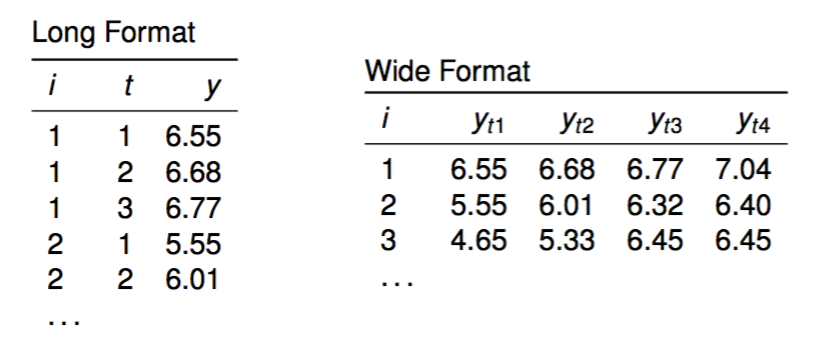
\includegraphics{figs/longwide.png}
\caption{\(i\) indiziert Einheiten, \(t\) indiziert Messzeitpunkte, \(y\) ist eine Variable}
\end{figure}

\begin{itemize}
\item
  Die Modelle in diesem Workshop nutzen das \emph{long format}
\item
  Datensätze können von einem ins andere Format transformiert werden, z.B. im \texttt{tidyverse}:

  \begin{itemize}
  \tightlist
  \item
    \texttt{tidyr::gather()} und \texttt{tidyr::spread()} (verwende ich in \texttt{R/data.R}) oder
  \item
    \texttt{tidyr::pivot\_longer()} und \texttt{tidyr::pivot\_wider()}
  \end{itemize}
\end{itemize}

\hypertarget{beispiel-daten}{%
\section{Beispiel-Daten}\label{beispiel-daten}}

\begin{itemize}
\item
  Titel: Soziale Normen im alltäglichen Umgang mit den Konsequenzen der Corona-Krise
\item
  sponsored by Jule Scheper und Sophie Bruns
\item
  Thema der Erhebung: Die Corona-Pandemie hat Regierungen auf der ganzen Welt dazu veranlasst, Reglungen zur Reduzierung der raschen Ausbreitung des Virus einzuführen. Die deutsche Bundesregierung hat am 22. März 2020 mehrere Maßnahmen zur Einschränkung sozialer Kontakte beschlossen. Diese Einschränkungen im sozialen Leben sind vollkommen neu und jede*r Einzelne muss sich auf diese Regelungen und die neue Lebenssituation einstellen. Diese Studie beschäftigt sich mit der Frage, wie Menschen sich im Alltag mit der Corona-Pandemie beschäftigen und wie sie mit den Regelungen zur Beschränkung sozialer Kontakte umgehen. Im Mittelpunkt der Untersuchung steht die Entstehung und Veränderung von sozialen Normen und persönlichen Einstellungen zur Beschränkung sozialer Kontakte über die Zeit.
\item
  Im Rahmen des Workshops steht der Einfluss der sozialen Normen und der eigenen Einstellung zum Verhalten auf das tatsächliche Social Distancing-Verhalten im Mittelpunkt.
\item
  Zeitraum der Erhebung: 1.4.-28.4.2020
\item
  Datum der Messzeitpunkte: Die Befragung besteht aus vier Wellen. Jede Welle war für eine Woche im Feld und bezog sich immer auf die vorherige Kalenderwoche.

  \begin{itemize}
  \tightlist
  \item
    Welle 1: Erhebungszeitraum vom 1.4.-7.4., Bezugszeitraum vom 23.3. bis 29.4.
  \item
    Welle 2: Erhebungszeitraum vom 8.4.-14.4., Bezugszeitraum vom 30.3. bis 5.4.
  \item
    Welle 3: Erhebungszeitraum vom 15.4.-21.4., Bezugszeitraum vom 6.4. bis 12.4.
  \item
    Welle 4: Erhebungszeitraum vom 22.4.-28.4., Bezugszeitraum vom 13.4. bis 19.4.
  \end{itemize}
\item
  Nachvollziehen der Aufbereitung in \texttt{R/data.R}
\item
  Direkt laden (z.B. für Übungen) aus \texttt{R/data/data.rds}
\item
  Der Datensatz ist bereits im \emph{long format}. \texttt{IDsosci} ist der Indikator für die Person, \texttt{wave} ist der Indikator für die Erhebungswelle.
\end{itemize}

\hypertarget{inhaltliche-variablen-im-datensatz}{%
\subsection*{Inhaltliche Variablen im Datensatz}\label{inhaltliche-variablen-im-datensatz}}
\addcontentsline{toc}{subsection}{Inhaltliche Variablen im Datensatz}

\begin{itemize}
\tightlist
\item
  Alter, Geschlecht (Dummy für weiblich), Bildung und Kollektivismus sind konstante Personenmerkmale.
\item
  Alle übrigen Variablen wurden in den vier Wellen wiederholt gemessen (mit Ausnahme von \texttt{desnorm4}, \texttt{injnorm4}, \texttt{verh4-6}, \texttt{verhint4-6}, die erst ab Welle 2 erfasst wurden).
\end{itemize}

\begin{tabular}{l|l}
\hline
Variablenname & Label\\
\hline
alter & Alter\\
\hline
besorg1 & Ich bin besorgt, wenn ich an Corona denke.\\
\hline
bildung & Bildungsabschluss\\
\hline
desnormp1 & …sind in der letzten Woche rausgegangen, auch wenn es sich nicht um einen Arztbesuch, Arbeitsweg, Spaziergang/Sport, Einkauf oder Hilfestellungen handelte.\\
\hline
desnormp2 & …haben sich in der letzten Woche in ihrer Freizeit mit mehr als einer anderen Person getroffen, die nicht im gleichen Haushalt lebt.\\
\hline
desnormp3 & …haben in der letzten Woche weniger als 1,5 Meter Abstand zu Personen gehalten, die nicht im gleichen Haushalt leben.\\
\hline
desnormp4 & ...haben sich in der letzten Woche strikt an die Maßnahmen zur Beschränkung sozialer Kontakte gehalten.\\
\hline
ein1 & Ich finde es in Ordnung, wenn man rausgeht, auch wenn es sich nicht um einen Arztbesuch, Arbeitsweg, Spaziergang/Sport, Einkauf oder Hilfe handelt.\\
\hline
ein2 & Ich finde es in Ordnung, wenn man sich in seiner Freizeit mit mehr als einer anderen Person trifft, die nicht im gleichen Haushalt lebt.\\
\hline
ein3 & Ich finde es in Ordnung, wenn man weniger als 1,5 Meter Abstand zu Personen hält, die nicht im gleichen Haushalt leben.\\
\hline
ein4 & Ich finde es wichtig, dass die Empfehlung zur Beschränkung sozialer Kontakte strikt eingehalten werden.\\
\hline
ein5 & Ich finde es richtig, dass generell Abstand gehalten werden soll.\\
\hline
injnormp1 & …finden es in Ordnung, wenn man rausgeht, auch wenn es sich nicht um einen Arztbesuch, Arbeitsweg, Spaziergang/Sport, Einkauf oder Hilfestellungen handelt.\\
\hline
injnormp2 & … finden es in Ordnung, wenn man sich in seiner Freizeit mit mehr als einer anderen Person trifft, die nicht im gleichen Haushalt lebt.\\
\hline
injnormp3 & …finden es in Ordnung, wenn man weniger als 1,5 Meter Abstand zu Personen hält, die nicht im gleichen Haushalt leben.\\
\hline
injnormp4 & ...finden es in Ordnung, wenn man sich strikt an die Maßnahmen zur Beschränkung sozialer Kontakte hält.\\
\hline
kompeer\_s1 & Freunde\\
\hline
kompeer\_s2 & Familie und Partner oder Partnerin\\
\hline
kompeer\_s3 & Bekannte (z.B. Arbeitskollegen und -kolleginnen, Vereinsmitglieder)\\
\hline
kompeer\_s4 & Prominente und/oder Influencer\\
\hline
med1 & Zeitungen \& Zeitschriften (z.B. Die ZEIT, Bild, Focus, der Spiegel)\\
\hline
med2 & Öffentlich-rechtliche Fernsehsender (z.B. ARD, ZDF, h1)\\
\hline
med3 & Private Fernsehsender (z.B. RTL, ProSieben)\\
\hline
med4 & Öffentlich-Rechtliche Radiosender (z.B. DLF, n-joy, NDR)\\
\hline
med5 & Private Radiosender (z.B. 89.0 RTL, ffn)\\
\hline
sex & Geschlecht W4 dummy\\
\hline
stress & Ich fühle mich durch die Corona-Pandemie gestresst.\\
\hline
verh1 & Ich bin rausgegangen, auch wenn es sich nicht um einen Arztbesuch, Arbeitsweg, Einkauf, Spaziergang/Sport oder Hilfestellung gehandelt hat.\\
\hline
verh2 & Ich habe mich mit mehr als einer Person getroffen, die nicht in meinem Haushalt lebt.\\
\hline
verh3 & Ich habe weniger 1,5 Meter Abstand zu Personen gehalten, die nicht in meinem Haushalt leben.\\
\hline
verh4 & Ich habe mich strikt an die Maßnahmen zur Beschränkung sozialer Kontakte gehalten.\\
\hline
verh5 & Ich habe mich im Privaten mit Freunden oder Familienmitgliedern getroffen, die nicht in meinem Haushalt leben.\\
\hline
verh6 & Ich war länger draußen als für einen üblichen Spaziergang (z.B. saß auf der Wiese oder am See).\\
\hline
verhint1 & Rausgehen, auch wenn es sich nicht um einen Arztbesuch, Arbeitsweg, Einkauf, Spaziergang/Sport oder Hilfestellung handelt.\\
\hline
verhint2 & Mich mit mehr als einer Person treffen, die nicht in meinem Haushalt lebt.\\
\hline
verhint3 & Weniger als 1,5 Meter Abstand zu Personen halten, die nicht in meinem Haushalt leben.\\
\hline
verhint4 & Mich strikt an die Maßnahmen zur Beschränkung sozialer Kontakte halten.\\
\hline
verhint5 & Mich im Privaten mit Freunden oder Familienmitgliedern treffen, die nicht in meinem Haushalt leben.\\
\hline
verhint6 & Mich länger draußen aufhalten als für einen üblichen Spaziergang (z.B. auf der Wiese oder am See sitzen).\\
\hline
veruns & Ich bin verunsichert durch die Corona-Krise.\\
\hline
\end{tabular}

\hypertarget{pooled-ols-wrong}{%
\section{Pooled OLS (WRONG!)}\label{pooled-ols-wrong}}

\begin{itemize}
\tightlist
\item
  Als erstes Beispiel wollen wir uns einer klassischen Frage aus der Theory of Planned Behavior zuwenden. Wir interessieren uns für den Effekt der Verhaltensintention auf das (berichtete) Verhalten (schließlich würden wir zum Start des Workshops ja gerne etwas finden ;)). Konkret betrachten wir den Effekt des Vorhabens, entgegen der Empfehlungen ohne relevanten Grund die Wohnung zu verlassen, auf den Selbstbericht, dies auch zu tun. Die beiden relevanten Variablen sind \texttt{verh1} und \texttt{verhint1}. Höhere Werte bedeuten eine häufigere Ausübung des Verhaltens bzw. eine höhere Wahrscheinlichkeit, das Verhalten auszuüben (gemessen auf Skala von 1 bis 5).
\item
  Die Abbildung zeigt die Entwicklung der beiden Variablen über die vier Wellen für 10 zufällig ausgewählte Personen.
\end{itemize}

\begin{Shaded}
\begin{Highlighting}[]
\NormalTok{id_smple =}\StringTok{ }\KeywordTok{sample}\NormalTok{(}\KeywordTok{unique}\NormalTok{(d}\OperatorTok{$}\NormalTok{IDsosci), }\DecValTok{10}\NormalTok{)}

\NormalTok{d }\OperatorTok\StringTok{ }\KeywordTok{filter}\NormalTok{(IDsosci }\OperatorTok\StringTok{ }\NormalTok{id_smple) }\OperatorTok\StringTok{ }\KeywordTok{select}\NormalTok{(IDsosci, wave, verh1, verhint1) }\OperatorTok\StringTok{ }
\StringTok{    }\KeywordTok{gather}\NormalTok{(variable, value, }\OperatorTok{-}\NormalTok{IDsosci, }\OperatorTok{-}\NormalTok{wave) }\OperatorTok\StringTok{ }\KeywordTok{ggplot}\NormalTok{(}\KeywordTok{aes}\NormalTok{(wave, value, }\DataTypeTok{group =}\NormalTok{ IDsosci, }
    \DataTypeTok{color =}\NormalTok{ IDsosci)) }\OperatorTok{+}\StringTok{ }\KeywordTok{geom_line}\NormalTok{(}\DataTypeTok{position =} \KeywordTok{position_jitter}\NormalTok{(}\DataTypeTok{height =} \FloatTok{0.1}\NormalTok{, }\DataTypeTok{width =} \DecValTok{0}\NormalTok{), }
    \DataTypeTok{show.legend =} \OtherTok{FALSE}\NormalTok{) }\OperatorTok{+}\StringTok{ }\KeywordTok{facet_wrap}\NormalTok{(}\StringTok{"variable"}\NormalTok{)}
\end{Highlighting}
\end{Shaded}

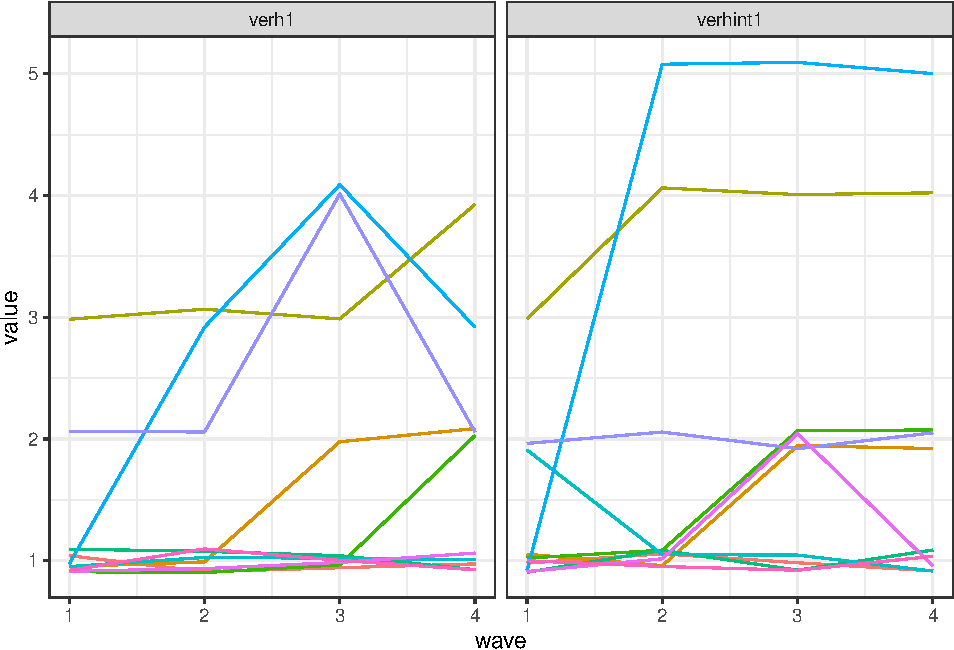
\includegraphics{workshop_panel_files/figure-latex/vis-ex1-1.pdf}

\begin{itemize}
\tightlist
\item
  Das einfachste Modell, diesen Effekt zu schätzen, ist eine einfache OLS Regression der Verhaltensintention auf das Verhalten.
\end{itemize}

\begin{Shaded}
\begin{Highlighting}[]
\KeywordTok{lm}\NormalTok{(verh1 }\OperatorTok{~}\StringTok{ }\NormalTok{verhint1, }\DataTypeTok{data =}\NormalTok{ d) }\OperatorTok\StringTok{ }\KeywordTok{tidy}\NormalTok{() }\OperatorTok\StringTok{ }\KeywordTok{mutate_if}\NormalTok{(is.numeric, round, }\DecValTok{2}\NormalTok{)}
\end{Highlighting}
\end{Shaded}

\begin{verbatim}
## # A tibble: 2 x 5
##   term        estimate std.error statistic p.value
##   <chr>          <dbl>     <dbl>     <dbl>   <dbl>
## 1 (Intercept)     0.46      0.02      19.2       0
## 2 verhint1        0.59      0.01      53.8       0
\end{verbatim}

\begin{itemize}
\tightlist
\item
  Das Modell besagt, dass die Häufigkeit, ohne triftigen Grund raus zu gehen, mit jedem Punkt auf der Intentionsskala um ca. \(b_{verhint1} = 0.6\) Punkte steigt.
\end{itemize}

\hypertarget{warum-ist-pooled-ols-immer-falsch-statistische-theorie}{%
\subsection*{Warum ist Pooled OLS immer falsch? Statistische Theorie}\label{warum-ist-pooled-ols-immer-falsch-statistische-theorie}}
\addcontentsline{toc}{subsection}{Warum ist Pooled OLS immer falsch? Statistische Theorie}

\begin{itemize}
\tightlist
\item
  Wir nennen dieses Modell \emph{pooled} OLS, da alle Beobachtungen einfach zusammengeworfen werden, ohne zu beachten, dass einige von ihnen zusammen gehören, da sie von denselben Personen stammen.
\end{itemize}

\begin{enumerate}
\def\labelenumi{\arabic{enumi})}
\tightlist
\item
  Exogenitätsannahme ist verletzt, \(E(u_i|x_i) \neq 0\)

  \begin{itemize}
  \tightlist
  \item
    Korrelationen zwischen den Variablen \(x\) gehen auf nicht gemessene Eigenschaften der Einheiten zurück, z.B. Eigenschaften der Person \(z_i\), die sowohl \(x_i\) als auch \(y_i\) beeinflussen.
  \item
    Auch bekannt als \emph{omitted variable bias}
  \item
    Könnte behoben werden, wenn alle \(z_i\) im Modell wären; diese Idee wird später wichtig
  \end{itemize}
\item
  Annahmen Homoskedastizität und unkorrelierte Residuen sind (wahrscheinlich) verletzt

  \begin{itemize}
  \tightlist
  \item
    Systematische Variation der Residuen zwischen Einheiten
  \item
    Wahrscheinlich serielle Korreationen durch die zeitliche Abhängigkeit der Messungen
  \end{itemize}
\item
  Annahme der Unabhängigkeit der Bebobachtungen verletzt

  \begin{itemize}
  \tightlist
  \item
    Überschätzung der Information von abhängigen Fällen (dieselbe Information ist mehrmals im Datensatz)

    \begin{itemize}
    \tightlist
    \item
      Zu kleine Standardfehler, zu große Zahl der Freiheitsgrade in Signifikanz-Tests
    \end{itemize}
  \item
    Die wahre Fallzahl (effective sample size) ist kleiner als Zahl der Zeilen im Datensatz (\emph{long format})
  \end{itemize}
\end{enumerate}

\hypertarget{warum-ist-pooled-ols-immer-falsch-inhaltliche-uxfcberlegungen}{%
\subsection*{Warum ist pooled OLS immer falsch? Inhaltliche Überlegungen}\label{warum-ist-pooled-ols-immer-falsch-inhaltliche-uxfcberlegungen}}
\addcontentsline{toc}{subsection}{Warum ist pooled OLS immer falsch? Inhaltliche Überlegungen}

\begin{itemize}
\tightlist
\item
  Unser Ziel ist es, den wahren kausalen Effekt von \(X\) auf \(Y\) zu schätzen.
\item
  Pooled OLS vermischt aber zwei Quellen von Unterschieden in den Daten: Den (kausalen) Effekt innerhalb der Personen (within) und die Unterschiede zwischen Personen (between).
\item
  Within und between Effekte können sich in Größe und sogar in der Richtung unterscheiden!
\item
  Die Schätzung aus einem poold OLS Modell vermischt den kausalen Effekt und die interindividuellen Unterschiede.
\item
  In der Sprache von Interventionsstudien ist das ein Selbstselektions-Problem: Was passiert, wenn Personen, die vor dem Treatment \(x\) schon höhere Werte in \(y\) haben, das Treatment häufiger auswählen als Personen, die niedrig in \$x§ sind?
\item
  Außerdem fällt auf, dass im einfachen OLS Modell nichts darauf hindeutet, dass es sich um Paneldaten handelt. Selbst wenn wir die genannten Probleme nicht hätten, hätten wir auch nichts durch die Paneldaten gewonnen.
\end{itemize}

\hypertarget{pooled-ols-within-und-between---eine-illustration}{%
\subsection*{Pooled OLS, within und between - eine Illustration}\label{pooled-ols-within-und-between---eine-illustration}}
\addcontentsline{toc}{subsection}{Pooled OLS, within und between - eine Illustration}

\begin{itemize}
\item
  Zum Abschluss noch ein imaginäres Beispiel, um den Unterschied von intraindividuellen (within) Effekten und interindividuellen Unterschieden zu verdeutlichen. Wir führen eine Panel-Studie mit acht Personen und sechs Messzeitpunkten zum Zusammenhang von Bier-Konsum und Hangover durch. Wir interessieren uns für die kausale Frage, ob mehr Bier zu einem schlimmeren Kater führt.
\item
  In der pooled OLS Analyse wird einfach die Rergressionsgerade durch alle Beobachung gelegt. Es zeigt sich ein negativer Zusammenhang. Je mehr Bier konsumiert wurde, desto schwächer fällt der Hangover aus.
\end{itemize}

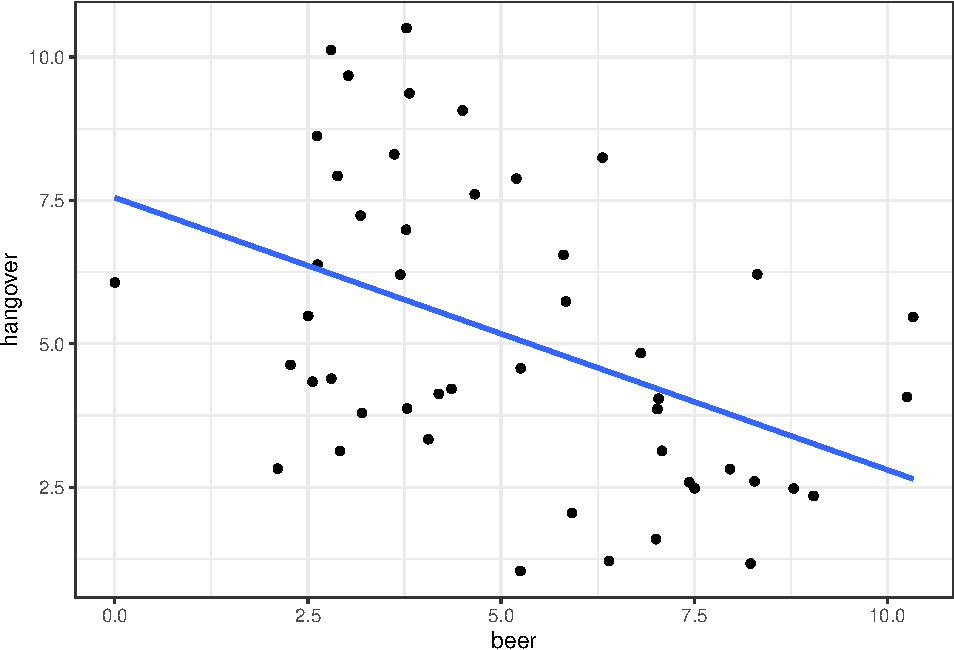
\includegraphics{workshop_panel_files/figure-latex/unnamed-chunk-8-1.pdf}

\begin{itemize}
\tightlist
\item
  Wenn wir aber für alle acht Personen separat den Zusammenhang zwischen Bierkonsum und Kater berechnen (so genanntes no pooling Modell), ergibt sich ein anderes Bild. Für alle Personen gilt mehr oder weniger deutlich: Je mehr Bier konsumiert wurde, desto stärker fällt der Hangover aus (within).
\end{itemize}

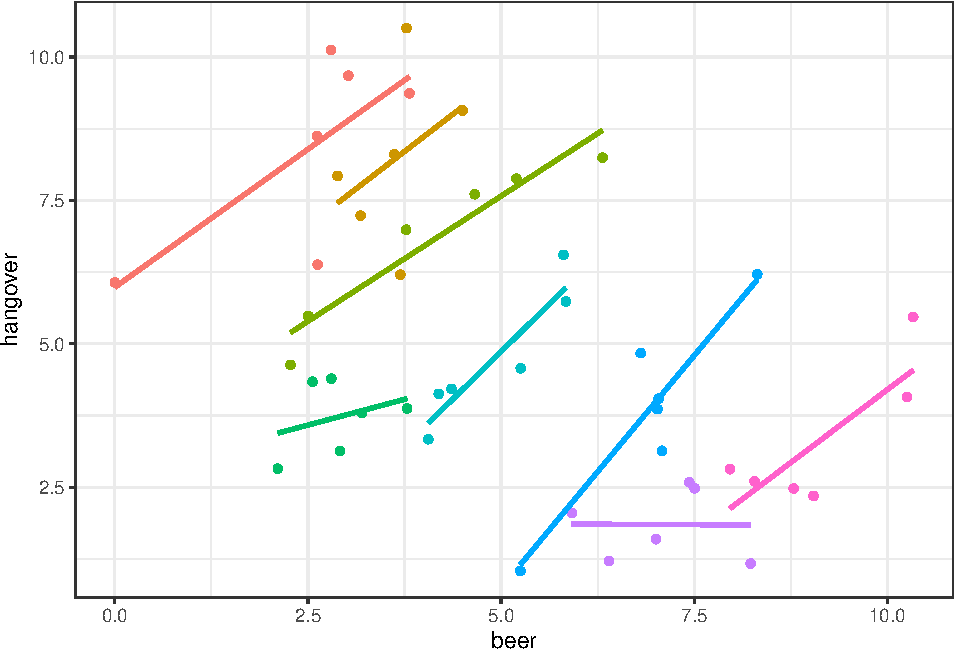
\includegraphics{workshop_panel_files/figure-latex/unnamed-chunk-9-1.pdf}

\begin{itemize}
\item
  Dazu kommt ein systematischer Unterschied zwischen den Personen (between): Personen, die im Durchschnitt mehr Bier trinken, haben im Durchschnitt einen schwächeren Hangover. Dies könnte auf eine nicht beobachte Drittvariable auf Ebene der Personen zurück gehen:

  \begin{itemize}
  \tightlist
  \item
    Vielleicht trinken Personen, die wissen, dass sie nicht so anfällig für einen Hangover sind, mehr, während Personen, die immer einen starken Kater haben, schon aus Angst vor dem nächsten Tag weniger trinken.
  \item
    Oder es ist ein Gewöhnungseffekt: Personen, die häufig viel trinken, gewöhnen sich an den Kater und nehmen ihn als weniger schlimm wahr. Oder mit Lemmy: ``A kid once said to me ``Do you get hangovers?'' I said, ``To get hangovers you have to stop drinking.''"
  \end{itemize}
\item
  Mit den vorliegenden Daten können wir die Frage nach dem Prozess nicht beantworten, da wir die Drittvariable nicht gemessen haben. Wir können aber \emph{alle} Variablen kontrollieren, die auf Personenebene liegen, z.B., indem wir wie in der Abbildung für jede Person ein separates Modell schätzen. Dann können Unterschiede zwischen den Einheiten per Modelldefinition keinen Einfluss auf die Schätzung haben. Etwas ähnliches passiert im \emph{fixed effects} Modell, das wir im nächsten Abschnitt besprechen.
\item
  An diesem Beispiel lässt sich übrigens auch schön sehen, warum uns Querschnittsdaten nicht bei der Identifikation kausaler Effekte helfen, wenn wir nicht für \(Z\) kontrollieren können. Wenn wir jede Panel-Welle für sich ananlysieren (die Daten also als unabhängige Querschnittserhebungen behandeln), finden wir jeweils einen negativen Zusammenhang zwischen Bierkonsum und Hangover.
\end{itemize}

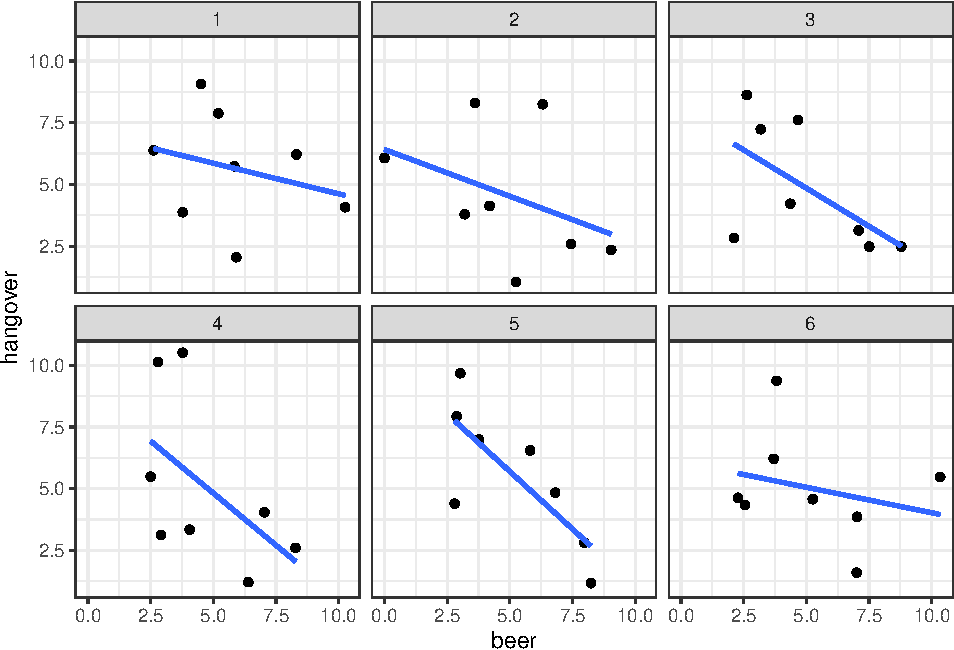
\includegraphics{workshop_panel_files/figure-latex/unnamed-chunk-10-1.pdf}

\hypertarget{fixed-effects-modelle}{%
\chapter{Fixed effects Modelle}\label{fixed-effects-modelle}}

\hypertarget{konzeptionelle-einfuxfchrung}{%
\section{Konzeptionelle Einführung}\label{konzeptionelle-einfuxfchrung}}

\begin{itemize}
\tightlist
\item
  Im ersten Teil des Abschnitts zu \emph{fixed effects} Modellen beschäftigen wir uns mit den Grundlagen der Modellierung. Dazu nutzen wir \texttt{stats::lm()} (übliche OLS-Schätzung linearer Modelle in \texttt{R}).
\end{itemize}

\hypertarget{wie-kuxf6nnen-wir-den-kausalen-within-person-effekt-mit-paneldaten-schuxe4tzen}{%
\subsection*{Wie können wir den kausalen (within-person) Effekt mit Paneldaten schätzen?}\label{wie-kuxf6nnen-wir-den-kausalen-within-person-effekt-mit-paneldaten-schuxe4tzen}}
\addcontentsline{toc}{subsection}{Wie können wir den kausalen (within-person) Effekt mit Paneldaten schätzen?}

\begin{enumerate}
\def\labelenumi{\arabic{enumi})}
\tightlist
\item
  Separate OLS Modelle für jede Person schätzen und Koeffizienten mitteln (no pooling).
\item
  Alle \(X\) und \(Y\) Variablen um die Mittelwerte der Person zentrieren (within transformation).
\item
  Dummy-Variablen für jede Person in das Regressionsmodell aufnehmen (least squares dummy variables {[}LSDV{]} estimation).
\end{enumerate}

\begin{itemize}
\tightlist
\item
  Alle drei Varianten entfernen die (beobachteten und nicht beobachten,) über die Zeit konstanten Unterschiede zwischen den Personen.
\item
  Varianten 2 und 3 entsprechen dem klassischen \emph{fixed effects} Modell. Die Unterschiede zwischen den Personen werden kontrolliert, indem die personenspezifischen Mittelwerte vor der Schätzung entfernt werden (2) oder für jede Person im Modell geschätzt werden (3).

  \begin{itemize}
  \tightlist
  \item
    \(y_{it}-\bar{y_{i}} = (x_{it} - \bar{x_{i}})'\beta + (u_{it} - \bar{u_{i}})\) oder \(y_{it} = \beta' x_{it}' + \alpha_i + u_{it}\)
  \end{itemize}
\item
  In Variante 1 dürfen die kausalen within-person Effekte zwischen den Personen variieren. Unter der Annahme homogener Treatment-Effekte (entspricht der typischen Annahme im randomisierten Between-Subject-Experiment) entspricht das Ergebnis asymptotisch den Varianten 2 und 3.

  \begin{itemize}
  \tightlist
  \item
    Der Schätzer ist aber weniger effizient, da zufällige Unterschiede in den Effekten zwischen den Personen aufgegriffen werden.
  \item
    Im letzten Teil des Abschnitts zum within-between-Modell kommen wir auf diesen Punkt zurück, wenn wir die Annahme homogener Treatment-Effekte lockern.
  \end{itemize}
\end{itemize}

\hypertarget{no-pooling}{%
\subsection*{No pooling}\label{no-pooling}}
\addcontentsline{toc}{subsection}{No pooling}

\begin{Shaded}
\begin{Highlighting}[]
\NormalTok{d }\OperatorTok\StringTok{ }\KeywordTok{group_by}\NormalTok{(IDsosci) }\OperatorTok\StringTok{ }\KeywordTok{nest}\NormalTok{() }\OperatorTok\StringTok{ }\KeywordTok{mutate}\NormalTok{(}\DataTypeTok{mdls =} \KeywordTok{map}\NormalTok{(data, }\OperatorTok{~}\KeywordTok{tidy}\NormalTok{(}\KeywordTok{lm}\NormalTok{(verh1 }\OperatorTok{~}\StringTok{ }\NormalTok{verhint1, }
    \DataTypeTok{data =}\NormalTok{ .x)))) }\OperatorTok\StringTok{ }\KeywordTok{unnest}\NormalTok{(mdls) }\OperatorTok\StringTok{ }\KeywordTok{ungroup}\NormalTok{() }\OperatorTok\StringTok{ }\KeywordTok{select}\NormalTok{(}\OperatorTok{-}\NormalTok{data) }\OperatorTok\StringTok{ }\KeywordTok{na.omit}\NormalTok{() }\OperatorTok\StringTok{ }
\StringTok{    }\KeywordTok{filter}\NormalTok{(statistic }\OperatorTok{!=}\StringTok{ }\OtherTok{Inf}\NormalTok{) }\OperatorTok\StringTok{ }\KeywordTok{filter}\NormalTok{(term }\OperatorTok{==}\StringTok{ "verhint1"}\NormalTok{) }\OperatorTok\StringTok{ }\KeywordTok{mutate_if}\NormalTok{(is.numeric, }
\NormalTok{    round, }\DecValTok{2}\NormalTok{) }\OperatorTok\StringTok{ }\NormalTok{print }\OperatorTok\StringTok{ }\KeywordTok{summarise}\NormalTok{(}\DataTypeTok{estimate =} \KeywordTok{mean}\NormalTok{(estimate), }\DataTypeTok{std.error =} \KeywordTok{sqrt}\NormalTok{(}\KeywordTok{mean}\NormalTok{(std.error}\OperatorTok{^}\DecValTok{2}\NormalTok{)))  }\CommentTok{# simple approximation}
\end{Highlighting}
\end{Shaded}

\begin{verbatim}
## # A tibble: 232 x 6
##    IDsosci term     estimate std.error statistic p.value
##    <chr>   <chr>       <dbl>     <dbl>     <dbl>   <dbl>
##  1 050IPY  verhint1     1.25      0.56  2.24e+ 0    0.15
##  2 05J4R8  verhint1     0.45      0.18  2.50e+ 0    0.13
##  3 08BDZJ  verhint1     0.33      0.53  6.30e- 1    0.59
##  4 0EO9L2  verhint1     1.67      0.67  2.50e+ 0    0.13
##  5 0F5L9Z  verhint1     0         0.71  0.          1   
##  6 0KYYAJ  verhint1     0.45      0.18  2.50e+ 0    0.13
##  7 0ONV4O  verhint1     1         0     9.01e+15    0   
##  8 0ZCKB5  verhint1    -0.35      0.5  -6.90e- 1    0.56
##  9 114OWA  verhint1     0.33      0.33  1.00e+ 0    0.42
## 10 16YGN0  verhint1     0.5       0.25  2.00e+ 0    0.18
## # ... with 222 more rows
\end{verbatim}

\begin{verbatim}
## # A tibble: 1 x 2
##   estimate std.error
##      <dbl>     <dbl>
## 1    0.502     0.521
\end{verbatim}

\begin{itemize}
\tightlist
\item
  Wir erhalten für jede Person einen Schätzer mit Standardfehler. Wir können diese mitteln, um einen Schätzer des durchschnittlichen kausalen Effekts zu erhalten.
\item
  Wir müssen die Schätzer entfernen, bei denen es wegen eines perfekten Zusammenhangs oder wegen fehlender intraindividueller Varianz keine OLS Lösung gibt.
\end{itemize}

\hypertarget{within-transformation}{%
\subsection*{Within Transformation}\label{within-transformation}}
\addcontentsline{toc}{subsection}{Within Transformation}

\begin{itemize}
\tightlist
\item
  Wir ziehen von jedem Messwert den Personenmittelwert ab. In das Modell gehen dann die um den Personenmittelwert bereinigten Variablen ein.
\end{itemize}

\begin{Shaded}
\begin{Highlighting}[]
\NormalTok{d_wi =}\StringTok{ }\NormalTok{d }\OperatorTok\StringTok{ }\KeywordTok{select}\NormalTok{(IDsosci, verh1, verhint1) }\OperatorTok\StringTok{ }\KeywordTok{group_by}\NormalTok{(IDsosci) }\OperatorTok\StringTok{ }\KeywordTok{mutate}\NormalTok{(}\DataTypeTok{verh1_wi =}\NormalTok{ verh1 }\OperatorTok{-}\StringTok{ }
\StringTok{    }\KeywordTok{mean}\NormalTok{(verh1), }\DataTypeTok{verhint1_wi =}\NormalTok{ verhint1 }\OperatorTok{-}\StringTok{ }\KeywordTok{mean}\NormalTok{(verhint1)) }\OperatorTok\StringTok{ }\KeywordTok{ungroup}\NormalTok{()}

\NormalTok{d_wi }\OperatorTok\StringTok{ }\KeywordTok{select}\NormalTok{(}\OperatorTok{-}\NormalTok{IDsosci) }\OperatorTok\StringTok{ }\NormalTok{summary}
\end{Highlighting}
\end{Shaded}

\begin{verbatim}
##      verh1          verhint1        verh1_wi      verhint1_wi   
##  Min.   :1.000   Min.   :1.000   Min.   :-3.00   Min.   :-3.00  
##  1st Qu.:1.000   1st Qu.:1.000   1st Qu.:-0.25   1st Qu.:-0.25  
##  Median :1.000   Median :1.000   Median : 0.00   Median : 0.00  
##  Mean   :1.529   Mean   :1.804   Mean   : 0.00   Mean   : 0.00  
##  3rd Qu.:2.000   3rd Qu.:2.000   3rd Qu.: 0.00   3rd Qu.: 0.00  
##  Max.   :5.000   Max.   :5.000   Max.   : 3.00   Max.   : 3.00
\end{verbatim}

\begin{Shaded}
\begin{Highlighting}[]
\NormalTok{d_wi }\OperatorTok\StringTok{ }\KeywordTok{lm}\NormalTok{(verh1_wi }\OperatorTok{~}\StringTok{ }\NormalTok{verhint1_wi, }\DataTypeTok{data =}\NormalTok{ .) }\OperatorTok\StringTok{ }\KeywordTok{tidy}\NormalTok{() }\OperatorTok\StringTok{ }\KeywordTok{mutate_if}\NormalTok{(is.numeric, }
\NormalTok{    round, }\DecValTok{2}\NormalTok{)}
\end{Highlighting}
\end{Shaded}

\begin{verbatim}
## # A tibble: 2 x 5
##   term        estimate std.error statistic p.value
##   <chr>          <dbl>     <dbl>     <dbl>   <dbl>
## 1 (Intercept)     0         0.01       0         1
## 2 verhint1_wi     0.35      0.01      24.9       0
\end{verbatim}

\begin{itemize}
\tightlist
\item
  Intuitive Interpretation: Eine Abweichung vom Personen-Durchschnitt in \(X\) um einen Punkt führt zu einer Abweichung vom Personen-Durchschnitt in \(Y\) um \(b_{X}\) Punkte.
\item
  Hier: Wenn eine Person um einen Punkt wahrscheinlicher rausgehen möchte als üblich, dann wird sie 0.34 Punkte häufiger rausgehen (beides auf 5er Skalen).
\item
  Das ist durchaus ein bedeutsamer Effekt. Aber zur Erinnerung: Der naiven pooled OLS Schätzung zufolge war der Effekt fast doppelt so groß. Es scheint also auch einen Unterschied zwischen Personen zugeben. Personen, die im Durchschnitt wahrscheinlicher raus gehen wollen, gehen im Durchschnitt auf häufiger raus.
\end{itemize}

\hypertarget{least-squares-mit-dummy-variablen-lsdv}{%
\subsection*{Least Squares mit Dummy Variablen (LSDV)}\label{least-squares-mit-dummy-variablen-lsdv}}
\addcontentsline{toc}{subsection}{Least Squares mit Dummy Variablen (LSDV)}

\begin{itemize}
\tightlist
\item
  Es wird ein Dummy-Indiktator für jede \(n-1\)te Person in das Modell aufgenommen.
\end{itemize}

\begin{Shaded}
\begin{Highlighting}[]
\NormalTok{d }\OperatorTok\StringTok{ }\KeywordTok{lm}\NormalTok{(verh1 }\OperatorTok{~}\StringTok{ }\NormalTok{verhint1 }\OperatorTok{+}\StringTok{ }\KeywordTok{factor}\NormalTok{(IDsosci), }\DataTypeTok{data =}\NormalTok{ .) }\OperatorTok\StringTok{ }\KeywordTok{tidy}\NormalTok{() }\OperatorTok\StringTok{ }\KeywordTok{mutate_if}\NormalTok{(is.numeric, }
\NormalTok{    round, }\DecValTok{2}\NormalTok{) }\OperatorTok\StringTok{ }\KeywordTok{print}\NormalTok{(}\DataTypeTok{n =} \DecValTok{17}\NormalTok{)}
\end{Highlighting}
\end{Shaded}

\begin{verbatim}
## # A tibble: 577 x 5
##    term                  estimate std.error statistic p.value
##    <chr>                    <dbl>     <dbl>     <dbl>   <dbl>
##  1 (Intercept)              0.65       0.28      2.31    0.02
##  2 verhint1                 0.35       0.02     21.5     0   
##  3 factor(IDsosci)02E6C8   -0.35       0.4      -0.86    0.39
##  4 factor(IDsosci)050IPY    1.21       0.4       3.01    0   
##  5 factor(IDsosci)05J4R8    0.32       0.4       0.79    0.43
##  6 factor(IDsosci)08BDZJ    0.96       0.4       2.39    0.02
##  7 factor(IDsosci)0BHGLF    0.570      0.4       1.42    0.16
##  8 factor(IDsosci)0EB6C1    0          0.4       0       1   
##  9 factor(IDsosci)0EO9L2    1.95       0.4       4.82    0   
## 10 factor(IDsosci)0F5L9Z    1.64       0.4       4.06    0   
## 11 factor(IDsosci)0KAKHF    2.2        0.4       5.44    0   
## 12 factor(IDsosci)0KYYAJ   -0.01       0.4      -0.02    0.98
## 13 factor(IDsosci)0ONV4O    0.33       0.4       0.82    0.41
## 14 factor(IDsosci)0PKFWT   -0.09       0.4      -0.22    0.83
## 15 factor(IDsosci)0ZCKB5    0.32       0.4       0.79    0.43
## 16 factor(IDsosci)114OWA    0.33       0.4       0.82    0.41
## 17 factor(IDsosci)11KVRK   -0.17       0.4      -0.43    0.67
## # ... with 560 more rows
\end{verbatim}

\begin{itemize}
\tightlist
\item
  Der Punktschätzer \(b_{X}\) entspricht genau dem Punktschätzer nach der within-person Transformation.
\item
  Zusätzlich gibt die Regressionskonstante den Mittelwert für Person 1 an und die \(n - 1\) Koeffizienten der Dummy-Variablen die Abweichung der übrigen Personen von diesem Mittelwert. Es gelten die üblichen Regeln für die Interpretation solcher Koeffizienten.
\end{itemize}

\hypertarget{welche-modellspezifikation-soll-ich-nutzen}{%
\subsection*{Welche Modellspezifikation soll ich nutzen?}\label{welche-modellspezifikation-soll-ich-nutzen}}
\addcontentsline{toc}{subsection}{Welche Modellspezifikation soll ich nutzen?}

\begin{enumerate}
\def\labelenumi{\arabic{enumi})}
\item
  Der Schätzer des durchschnittlichen kausalen Effekts in der no pooling Spezifikation ist im Vergleich zu den beiden anderen Varianten weniger effizient. Außerdem ist er praktisch schwieriger zu ermitteln, da er erst aus den Schätzern der Einzel-Modelle berechnet werden muss. Wenn wir die Annahme eines homogenen kausalen Effekts treffen (und das tun wir üblicherweise), dann gibt es keinen Grund, das no pooling Modell in der Praxis zu verwenden.
\item
  Die Spezifikationen mit within-person Transformation und LSDV ergeben dieselben Punktschätzer für den kausalen Effekt und sind insofern austauschbar.
\item
  Die Standardfehler des Modells mit einer naiven within-person Transformation (wie oben dargestellt) sind zu klein, da wir die Stichprobenmittelwerte und nicht die (mit Unsicherheit behafteten) Schätzer der Populationsmittelwerte zur Zentrierung verwenden. Die Standardfehler müssen daher angepasst werden (passiert in spezialisierten Software-Paketen automatisch).
\item
  Die LSDV Spezifikation ist in fast jedem Softwarepaket einfach umzusetzen. Mit großen Datensätzen wird aber die Schätzung langsam und der Output unübersichtlich.
\end{enumerate}

\begin{itemize}
\item
  Unabhängig von der Spezifikation gelten weiterhin alle Annahmen der (OLS) Regression. Besonders gern vergessen wird der \emph{omitted variable bias} durch nicht gemessene, über die Zeit variierdene \(Z\). \emph{Fixed effects} Modelle kontrollieren nur die \(Z\), die auf konstante Merkmale der als \emph{fixed effects} spezifizierten Einheiten zurückgehen.
\item
  Insgesamt sind viele quantitative Sozialforscher (v.a. die mit einer Ökonometrie-Ausbildung) der Ansicht, dass \emph{fixed effects} Modelle die beste Methode sind, um kausale Effekte aus nicht-experimentellen Daten zu schätzen.
\end{itemize}

\hypertarget{mehre-fixed-effects-in-einem-modell-perioden-effekte}{%
\subsection*{Mehre fixed effects in einem Modell -- Perioden-Effekte}\label{mehre-fixed-effects-in-einem-modell-perioden-effekte}}
\addcontentsline{toc}{subsection}{Mehre fixed effects in einem Modell -- Perioden-Effekte}

\begin{itemize}
\tightlist
\item
  Grundsätzlich können in einem Modell beliebig viele \emph{fixed effects} spezifiziert werden.
\item
  In Paneldaten ist der Erhebungszeitpunkt bzw. die Ergebungsperiode (Panelwelle) eine typische Variable, über die verschiedene, für alle Personen konstante Effekte kontrolliert werden können.
\item
  Einige Lehrbücher empfehlen, dies \emph{immer} zu tun, da kausale Effekte von Ereignissen, die für alle Einheiten konstant sind, statistisch nicht identifiziert sind.
\item
  Eine typische Spezifikation ist die Aufnahme eines \emph{fixed effects} für den Indikator der Panelwelle.
\item
  In der LSDV-Spezifikation kann einfach ein weiterer Dummy-Faktor hinzugefügt werden. Die within-person Transformation ist mathematisch komplizierter, wird aber in spezialisierten Software-Pakten im Hintergrund erledigt. Es können auch beide Spezifikationen kombiniert werden, wenn z.B. die Periodeneffekte von inhaltlichem Interesse sind und im Output angezeigt werden sollen (siehe nächsten Teilabschnitt).
\end{itemize}

\hypertarget{ein-beispiel-mit-fixed-effects-fuxfcr-personen-und-perioden}{%
\subsection*{\texorpdfstring{Ein Beispiel mit \emph{fixed effects} für Personen und Perioden}{Ein Beispiel mit fixed effects für Personen und Perioden}}\label{ein-beispiel-mit-fixed-effects-fuxfcr-personen-und-perioden}}
\addcontentsline{toc}{subsection}{Ein Beispiel mit \emph{fixed effects} für Personen und Perioden}

\begin{Shaded}
\begin{Highlighting}[]
\NormalTok{d }\OperatorTok\StringTok{ }\KeywordTok{lm}\NormalTok{(verh1 }\OperatorTok{~}\StringTok{ }\NormalTok{verhint1 }\OperatorTok{+}\StringTok{ }\KeywordTok{factor}\NormalTok{(wave) }\OperatorTok{+}\StringTok{ }\KeywordTok{factor}\NormalTok{(IDsosci), }\DataTypeTok{data =}\NormalTok{ .) }\OperatorTok\StringTok{ }\KeywordTok{tidy}\NormalTok{() }\OperatorTok\StringTok{ }
\StringTok{    }\KeywordTok{mutate_if}\NormalTok{(is.numeric, round, }\DecValTok{2}\NormalTok{) }\OperatorTok\StringTok{ }\KeywordTok{print}\NormalTok{(}\DataTypeTok{n =} \DecValTok{17}\NormalTok{)}
\end{Highlighting}
\end{Shaded}

\begin{verbatim}
## # A tibble: 580 x 5
##    term                  estimate std.error statistic p.value
##    <chr>                    <dbl>     <dbl>     <dbl>   <dbl>
##  1 (Intercept)               0.6       0.28      2.13    0.03
##  2 verhint1                  0.33      0.02     19.8     0   
##  3 factor(wave)2             0.02      0.03      0.6     0.55
##  4 factor(wave)3             0.14      0.03      4.15    0   
##  5 factor(wave)4             0.12      0.03      3.41    0   
##  6 factor(IDsosci)02E6C8    -0.33      0.4      -0.83    0.41
##  7 factor(IDsosci)050IPY     1.26      0.4       3.15    0   
##  8 factor(IDsosci)05J4R8     0.34      0.4       0.85    0.39
##  9 factor(IDsosci)08BDZJ     1.01      0.4       2.53    0.01
## 10 factor(IDsosci)0BHGLF     0.59      0.4       1.48    0.14
## 11 factor(IDsosci)0EB6C1     0         0.4       0       1   
## 12 factor(IDsosci)0EO9L2     2.02      0.4       5.01    0   
## 13 factor(IDsosci)0F5L9Z     1.68      0.4       4.2     0   
## 14 factor(IDsosci)0KAKHF     2.27      0.4       5.63    0   
## 15 factor(IDsosci)0KYYAJ     0         0.4       0.01    0.99
## 16 factor(IDsosci)0ONV4O     0.34      0.4       0.84    0.4 
## 17 factor(IDsosci)0PKFWT    -0.08      0.4      -0.21    0.84
## # ... with 563 more rows
\end{verbatim}

\begin{itemize}
\tightlist
\item
  \(b_{verhint1}\) quantifiziert weiterhin den kausalen Effekt von Interesse. Er ist robust gegen die Kontrolle des Periodeneffekts.
\item
  Die \(b_{wave_t}\) zeigen den Kontrast zur ersten Welle. In diesem Fall sind liegen in der dritten und vierten Welle die Häufigkeiten des Rausgehens höher als noch in den ersten beiden Wellen.
\item
  Die \(b_{id_i}\) zeigen weiterhin den Kontrast zu Person 1 (substantiell nicht sonderlich interessant).
\end{itemize}

\hypertarget{uxfcbungsaufgaben-1}{%
\section{Übungsaufgaben 1}\label{uxfcbungsaufgaben-1}}

\begin{enumerate}
\def\labelenumi{\arabic{enumi})}
\tightlist
\item
  Schätze den kausalen Effekt der Informationshäufigkeit aus öffentlich-rechtlichen TV-Programmen (\texttt{med2}) auf die Intention, weniger als 1.5m Abstand zu einer Person zu halten, die nicht im eigenen Haushalt lebt (\texttt{verhint3}).

  \begin{itemize}
  \tightlist
  \item
    Schätze zuerst das \emph{falsche} pooled OLS Modell.
  \item
    Schätze dann das einfache \emph{fixed effects} Modell mit einer Spezifikation freier Wahl.
  \item
    Vergleiche schließlich die Modelle mit und ohne Periodeneffekt.
  \end{itemize}
\item
  Spezifiziere, schätze und interpretiere ein eigenes bivariates \emph{fixed effects} Modell mit Daten aus dem Beispieldatensatz.
\end{enumerate}

\hypertarget{fixed-effects-modelle-in-der-praktischen-anwendung}{%
\section{\texorpdfstring{\emph{Fixed effects} Modelle in der praktischen Anwendung}{Fixed effects Modelle in der praktischen Anwendung}}\label{fixed-effects-modelle-in-der-praktischen-anwendung}}

\begin{itemize}
\tightlist
\item
  Auch wenn wir das \emph{fixed effects} Modell nur mit \texttt{stats::lm()} und der LSDV-Spezifikation schätzen können, ist die weitere Arbeit mit diesen Modellen nicht ideal - besonders, wenn wir tiefer in Detail-Anpassungen einsteigen.
\item
  Zudem wird das Schätzen mit \texttt{stats::lm()} und LSDV bei großen Datensätzen und mit vielen \emph{fixed effects} langsam.
\item
  \texttt{plm} \citep{R-plm} ist das etablierte Paket für das Schätzen von ökonometrischen Panel-Modellen in \texttt{R}. Es bietet ein einfaches Interface zu allen Standardmodellen (und zu den übrigen Klassikern der Ökonometrie, instrumental variables, differences in differences).
\item
  Das Schätzen der Modelle basiert auf OLS mit Datentransformationen im Hintergrund. Dadurch ist das Schätzen wesentlich schneller als mit einer LSDV-Spezifikation. Die notwendigen Anpassungen der Standardfehler werden ebenfalls vorgenommen.
\end{itemize}

\hypertarget{spezifikation-eines-einfachen-fixed-effects-modells-mit-plm}{%
\subsection*{\texorpdfstring{Spezifikation eines einfachen \emph{fixed effects} Modells mit \texttt{plm}}{Spezifikation eines einfachen fixed effects Modells mit plm}}\label{spezifikation-eines-einfachen-fixed-effects-modells-mit-plm}}
\addcontentsline{toc}{subsection}{Spezifikation eines einfachen \emph{fixed effects} Modells mit \texttt{plm}}

\begin{itemize}
\tightlist
\item
  Das \emph{fixed effects} Modell wird über \texttt{model\ =\ "within"} angefordert. Mit \texttt{index\ =\ "IDsosci"} wird der Indikator für die Einheiten angegeben.
\end{itemize}

\begin{Shaded}
\begin{Highlighting}[]
\NormalTok{d }\OperatorTok\StringTok{ }\KeywordTok{plm}\NormalTok{(verh1 }\OperatorTok{~}\StringTok{ }\NormalTok{verhint1, }\DataTypeTok{data =}\NormalTok{ ., }\DataTypeTok{index =} \StringTok{"IDsosci"}\NormalTok{, }\DataTypeTok{model =} \StringTok{"within"}\NormalTok{) }\OperatorTok\StringTok{ }\KeywordTok{summary}\NormalTok{()}
\end{Highlighting}
\end{Shaded}

\begin{verbatim}
## Oneway (individual) effect Within Model
## 
## Call:
## plm(formula = verh1 ~ verhint1, data = ., model = "within", index = "IDsosci")
## 
## Balanced Panel: n = 576, T = 4, N = 2304
## 
## Residuals:
##      Min.   1st Qu.    Median   3rd Qu.      Max. 
## -3.000000 -0.163516  0.000000  0.095937  3.000000 
## 
## Coefficients:
##          Estimate Std. Error t-value  Pr(>|t|)    
## verhint1 0.345937   0.016061  21.539 < 2.2e-16 ***
## ---
## Signif. codes:  0 '***' 0.001 '**' 0.01 '*' 0.05 '.' 0.1 ' ' 1
## 
## Total Sum of Squares:    702.5
## Residual Sum of Squares: 553.75
## R-Squared:      0.21175
## Adj. R-Squared: -0.051155
## F-statistic: 463.924 on 1 and 1727 DF, p-value: < 2.22e-16
\end{verbatim}

\begin{itemize}
\tightlist
\item
  Der Output von \texttt{summary()} liefert eine korrekte Beschreibung der Fallzahlen im Datensatz.
\item
  Beachte: Das angepasste \(R^2\) ist hier (wie in vielen \emph{fixed effects} Modellen) negativ. Das ist kein Grund zur Beunruhigung. Die Logik dahinter kann gut nachvollzogen werden, wenn wir uns die LSDV-Spezifikation in Erinnerung rufen. Zusätzlich zu den inhaltlich relevanten Prädiktoren enthält das Modell \(n - 1\) Prädiktoren für die Einheiten.
\end{itemize}

\hypertarget{mehre-fixed-effects-in-einem-modell-perioden-effekte-mit-plm}{%
\subsection*{\texorpdfstring{Mehre \emph{fixed effects} in einem Modell -- Perioden-Effekte mit \texttt{plm}}{Mehre fixed effects in einem Modell -- Perioden-Effekte mit plm}}\label{mehre-fixed-effects-in-einem-modell-perioden-effekte-mit-plm}}
\addcontentsline{toc}{subsection}{Mehre \emph{fixed effects} in einem Modell -- Perioden-Effekte mit \texttt{plm}}

\begin{itemize}
\tightlist
\item
  \texttt{plm} bietet zwei Möglichkeiten, die Perioden-Effekte zu spezifizieren (identische Ergebnisse, anderer Output):
\end{itemize}

\begin{enumerate}
\def\labelenumi{\arabic{enumi})}
\tightlist
\item
  Zwei Indices \texttt{index=c("IDsosci",\ "wave")} und \texttt{effect\ =\ "twoways"} für die within-Transformation.

  \begin{itemize}
  \tightlist
  \item
    Es wird ``still'' für Personen und Perioden kontrolliert, beide werden nicht im Output angezeigt.
  \item
    Das \(R^2\) bezieht sich nur auf die Varianzaufklärung durch die Prädiktoren.
  \end{itemize}
\item
  Perioden-Effekt als Dummies hinzufügen.

  \begin{itemize}
  \tightlist
  \item
    Praktisch, wenn es nur wenige Perioden gibt und wir die Ergebnisse dazu direkt im Output sehen wollen.
  \item
    Das \(R^2\) bezieht sich auf die Varianzaufklärung durch die Prädiktoren und den Perioden-Effekt.
  \end{itemize}
\end{enumerate}

\begin{Shaded}
\begin{Highlighting}[]
\NormalTok{d }\OperatorTok\StringTok{ }\KeywordTok{plm}\NormalTok{(verh1 }\OperatorTok{~}\StringTok{ }\NormalTok{verhint1, }\DataTypeTok{data =}\NormalTok{ ., }\DataTypeTok{index =} \KeywordTok{c}\NormalTok{(}\StringTok{"IDsosci"}\NormalTok{, }\StringTok{"wave"}\NormalTok{), }\DataTypeTok{model =} \StringTok{"within"}\NormalTok{, }
    \DataTypeTok{effect =} \StringTok{"twoways"}\NormalTok{) }\OperatorTok\StringTok{ }\KeywordTok{summary}\NormalTok{()}
\end{Highlighting}
\end{Shaded}

\begin{verbatim}
## Twoways effects Within Model
## 
## Call:
## plm(formula = verh1 ~ verhint1, data = ., effect = "twoways", 
##     model = "within", index = c("IDsosci", "wave"))
## 
## Balanced Panel: n = 576, T = 4, N = 2304
## 
## Residuals:
##      Min.   1st Qu.    Median   3rd Qu.      Max. 
## -3.070526 -0.180571  0.011669  0.131626  3.049432 
## 
## Coefficients:
##          Estimate Std. Error t-value  Pr(>|t|)    
## verhint1 0.328779   0.016614  19.789 < 2.2e-16 ***
## ---
## Signif. codes:  0 '***' 0.001 '**' 0.01 '*' 0.05 '.' 0.1 ' ' 1
## 
## Total Sum of Squares:    669.68
## Residual Sum of Squares: 545.72
## R-Squared:      0.1851
## Adj. R-Squared: -0.088576
## F-statistic: 391.609 on 1 and 1724 DF, p-value: < 2.22e-16
\end{verbatim}

\begin{Shaded}
\begin{Highlighting}[]
\NormalTok{mdl_pfe_pdv =}\StringTok{ }\NormalTok{d }\OperatorTok\StringTok{ }\KeywordTok{plm}\NormalTok{(verh1 }\OperatorTok{~}\StringTok{ }\NormalTok{verhint1 }\OperatorTok{+}\StringTok{ }\KeywordTok{factor}\NormalTok{(wave), }\DataTypeTok{data =}\NormalTok{ ., }\DataTypeTok{index =} \StringTok{"IDsosci"}\NormalTok{, }
    \DataTypeTok{model =} \StringTok{"within"}\NormalTok{)}
\NormalTok{mdl_pfe_pdv }\OperatorTok\StringTok{ }\KeywordTok{summary}\NormalTok{()}
\end{Highlighting}
\end{Shaded}

\begin{verbatim}
## Oneway (individual) effect Within Model
## 
## Call:
## plm(formula = verh1 ~ verhint1 + factor(wave), data = ., model = "within", 
##     index = "IDsosci")
## 
## Balanced Panel: n = 576, T = 4, N = 2304
## 
## Residuals:
##      Min.   1st Qu.    Median   3rd Qu.      Max. 
## -3.070526 -0.180571  0.011669  0.131626  3.049432 
## 
## Coefficients:
##               Estimate Std. Error t-value  Pr(>|t|)    
## verhint1      0.328779   0.016614 19.7891 < 2.2e-16 ***
## factor(wave)2 0.019997   0.033589  0.5954 0.5516856    
## factor(wave)3 0.139955   0.033691  4.1540 3.426e-05 ***
## factor(wave)4 0.117763   0.034484  3.4150 0.0006526 ***
## ---
## Signif. codes:  0 '***' 0.001 '**' 0.01 '*' 0.05 '.' 0.1 ' ' 1
## 
## Total Sum of Squares:    702.5
## Residual Sum of Squares: 545.72
## R-Squared:      0.22318
## Adj. R-Squared: -0.037717
## F-statistic: 123.824 on 4 and 1724 DF, p-value: < 2.22e-16
\end{verbatim}

\hypertarget{robuste-standardfehler}{%
\subsection*{Robuste Standardfehler}\label{robuste-standardfehler}}
\addcontentsline{toc}{subsection}{Robuste Standardfehler}

\begin{itemize}
\item
  In der ökonometrischen Diskussion ist die Wahl der korrekten (robusten) Standardfehler sehr prominent. Diese sind robust gegen Verletzung verschiedener Annahmen, z.B. durch serielle Korrelationen der Residuen oder Heteroskedastizität.
\item
  Das \texttt{lmtest} Paket \citep{R-lmtest} ist kompatibel mit Modellen aus \texttt{plm}. Es implementiert zahlreiche robuste Schätzer bzw. Korrekturen.
\item
  Hier die ``normalen'' Standardfehler und bei Heteroskedastizität robuste Standardfehler sowie die darauf basierenden Konfidenzintervalle im Vergleich.
\item
  Weiter wollen wir dieses Thema hier nicht vertiefen. Ich empfehle für die Details der Umsetzung in \texttt{plm} \citet{plm2017} und zu einer kritischen Auseinandersetzung \citet{kingHowRobustStandard2015}.
\end{itemize}

\begin{Shaded}
\begin{Highlighting}[]
\CommentTok{# Normale SE und CI}
\NormalTok{mdl_pfe_pdv }\OperatorTok\StringTok{ }\KeywordTok{coeftest}\NormalTok{() }\OperatorTok\StringTok{ }\KeywordTok{round}\NormalTok{(}\DecValTok{3}\NormalTok{)}
\end{Highlighting}
\end{Shaded}

\begin{verbatim}
## 
## t test of coefficients:
## 
##               Estimate Std. Error t value Pr(>|t|)    
## verhint1         0.329      0.017  19.789   <2e-16 ***
## factor(wave)2    0.020      0.034   0.595    0.552    
## factor(wave)3    0.140      0.034   4.154   <2e-16 ***
## factor(wave)4    0.118      0.034   3.415    0.001 ***
## ---
## Signif. codes:  0 '***' 0.001 '**' 0.01 '*' 0.05 '.' 0.1 ' ' 1
\end{verbatim}

\begin{Shaded}
\begin{Highlighting}[]
\NormalTok{mdl_pfe_pdv }\OperatorTok\StringTok{ }\KeywordTok{coefci}\NormalTok{() }\OperatorTok\StringTok{ }\KeywordTok{round}\NormalTok{(}\DecValTok{3}\NormalTok{)}
\end{Highlighting}
\end{Shaded}

\begin{verbatim}
##                2.5 % 97.5 %
## verhint1       0.296  0.361
## factor(wave)2 -0.046  0.086
## factor(wave)3  0.074  0.206
## factor(wave)4  0.050  0.185
\end{verbatim}

\begin{Shaded}
\begin{Highlighting}[]
\CommentTok{# Heteroskedasticity-robust SE and CI}
\NormalTok{mdl_pfe_pdv }\OperatorTok\StringTok{ }\KeywordTok{coeftest}\NormalTok{(}\DataTypeTok{vcov. =}\NormalTok{ vcovHC) }\OperatorTok\StringTok{ }\KeywordTok{round}\NormalTok{(}\DecValTok{3}\NormalTok{)}
\end{Highlighting}
\end{Shaded}

\begin{verbatim}
## 
## t test of coefficients:
## 
##               Estimate Std. Error t value Pr(>|t|)    
## verhint1         0.329      0.028  11.868   <2e-16 ***
## factor(wave)2    0.020      0.029   0.688    0.491    
## factor(wave)3    0.140      0.036   3.849   <2e-16 ***
## factor(wave)4    0.118      0.032   3.701   <2e-16 ***
## ---
## Signif. codes:  0 '***' 0.001 '**' 0.01 '*' 0.05 '.' 0.1 ' ' 1
\end{verbatim}

\begin{Shaded}
\begin{Highlighting}[]
\NormalTok{mdl_pfe_pdv }\OperatorTok\StringTok{ }\KeywordTok{coefci}\NormalTok{(}\DataTypeTok{vcov. =}\NormalTok{ vcovHC) }\OperatorTok\StringTok{ }\KeywordTok{round}\NormalTok{(}\DecValTok{3}\NormalTok{)}
\end{Highlighting}
\end{Shaded}

\begin{verbatim}
##                2.5 % 97.5 %
## verhint1       0.274  0.383
## factor(wave)2 -0.037  0.077
## factor(wave)3  0.069  0.211
## factor(wave)4  0.055  0.180
\end{verbatim}

\hypertarget{aufnahme-weiterer-uxfcber-die-zeit-variierender-pruxe4diktoren}{%
\subsection*{Aufnahme weiterer über die Zeit variierender Prädiktoren}\label{aufnahme-weiterer-uxfcber-die-zeit-variierender-pruxe4diktoren}}
\addcontentsline{toc}{subsection}{Aufnahme weiterer über die Zeit variierender Prädiktoren}

\begin{itemize}
\item
  Die Aufnahme weiterer Prädiktoren, die über die Zeit variieren, erfolgt prinzipiell wie im bekannten OLS Modell.
\item
  Wichtig ist, dass es bei \emph{fixed effects} Modellen explizit um das Schätzen von kausalen Effekten geht. Entsprechend bedacht sollte die Auswahl von weiteren Prädiktoren sein. Ein ``kitchen sink'' Ansatz, den man vor allem in OLS mit Querschnittsdaten sieht, ist hier nicht angebracht. Es muss (wie eigentlich immer) darauf geachtet werden, welche Koeffizienten eines Regressionsmodells kausal interpretiert werden dürfen \citep{keeleCausalInterpretationEstimated2019}. Im \emph{fixed effects} Modell müssen wir uns das ganz explizit vergegenwärtigen und in der Ergebnisdarstellung berücksichtigen, da die Modellklasse kausale Effekte impliziert.
\item
  Nach der TPB dürfen wir dieses Modell annehmen, da die drei Prädiktoren auf derselben kausalen Stufe stehen: Verhaltensintention \textasciitilde{} Einstellung + Deskriptive Norm + Injunktive Norm. Hier schätzen wir das Modell für die Verhaltensintention \emph{Rausgehen ohne triftigen Grund}.
\end{itemize}

\begin{Shaded}
\begin{Highlighting}[]
\NormalTok{d }\OperatorTok\StringTok{ }\KeywordTok{plm}\NormalTok{(verhint1 }\OperatorTok{~}\StringTok{ }\NormalTok{ein1 }\OperatorTok{+}\StringTok{ }\NormalTok{desnormp1 }\OperatorTok{+}\StringTok{ }\NormalTok{injnormp1 }\OperatorTok{+}\StringTok{ }\KeywordTok{factor}\NormalTok{(wave), }\DataTypeTok{data =}\NormalTok{ ., }\DataTypeTok{index =} \StringTok{"IDsosci"}\NormalTok{, }
    \DataTypeTok{model =} \StringTok{"within"}\NormalTok{) }\OperatorTok\StringTok{ }\KeywordTok{tidy}\NormalTok{() }\OperatorTok\StringTok{ }\KeywordTok{mutate_if}\NormalTok{(is.numeric, round, }\DecValTok{2}\NormalTok{)}
\end{Highlighting}
\end{Shaded}

\begin{verbatim}
## # A tibble: 6 x 5
##   term          estimate std.error statistic p.value
##   <chr>            <dbl>     <dbl>     <dbl>   <dbl>
## 1 ein1              0.31      0.02     12.4     0   
## 2 desnormp1         0.05      0.03      1.56    0.12
## 3 injnormp1         0.1       0.03      3.31    0   
## 4 factor(wave)2     0.21      0.05      4.69    0   
## 5 factor(wave)3     0.24      0.05      5.3     0   
## 6 factor(wave)4     0.39      0.05      8.32    0
\end{verbatim}

\begin{itemize}
\tightlist
\item
  Vor allem die Einstellung zum Verhalten und die wahrgenommenen normativen Erwartungen haben stärkere kausale Effekte auf die Verhaltensintention.
\end{itemize}

\hypertarget{aufnahme-eines-personenmerkmals-funktioniert-nicht-ohne-warnung}{%
\subsection*{Aufnahme eines Personenmerkmals (funktioniert nicht, ohne Warnung!)}\label{aufnahme-eines-personenmerkmals-funktioniert-nicht-ohne-warnung}}
\addcontentsline{toc}{subsection}{Aufnahme eines Personenmerkmals (funktioniert nicht, ohne Warnung!)}

\begin{itemize}
\tightlist
\item
  In einer typischen Regresssionanalyse würden wir uns z.B. auch dafür interessieren, ob sich das Verhalten nach dem Geschlecht unterscheidet. Wir nehmen also \texttt{C\_sex} in die Formel auf, mit der wir das Modell in \texttt{plm} spezifizieren.
\end{itemize}

\begin{Shaded}
\begin{Highlighting}[]
\NormalTok{d }\OperatorTok\StringTok{ }\KeywordTok{plm}\NormalTok{(verh1 }\OperatorTok{~}\StringTok{ }\NormalTok{verhint1 }\OperatorTok{+}\StringTok{ }\NormalTok{C_sex }\OperatorTok{+}\StringTok{ }\KeywordTok{factor}\NormalTok{(wave), }\DataTypeTok{data =}\NormalTok{ ., }\DataTypeTok{index =} \StringTok{"IDsosci"}\NormalTok{, }\DataTypeTok{model =} \StringTok{"within"}\NormalTok{) }\OperatorTok\StringTok{ }
\StringTok{    }\NormalTok{summary}
\end{Highlighting}
\end{Shaded}

\begin{verbatim}
## Oneway (individual) effect Within Model
## 
## Call:
## plm(formula = verh1 ~ verhint1 + C_sex + factor(wave), data = ., 
##     model = "within", index = "IDsosci")
## 
## Balanced Panel: n = 576, T = 4, N = 2304
## 
## Residuals:
##      Min.   1st Qu.    Median   3rd Qu.      Max. 
## -3.070526 -0.180571  0.011669  0.131626  3.049432 
## 
## Coefficients:
##               Estimate Std. Error t-value  Pr(>|t|)    
## verhint1      0.328779   0.016614 19.7891 < 2.2e-16 ***
## factor(wave)2 0.019997   0.033589  0.5954 0.5516856    
## factor(wave)3 0.139955   0.033691  4.1540 3.426e-05 ***
## factor(wave)4 0.117763   0.034484  3.4150 0.0006526 ***
## ---
## Signif. codes:  0 '***' 0.001 '**' 0.01 '*' 0.05 '.' 0.1 ' ' 1
## 
## Total Sum of Squares:    702.5
## Residual Sum of Squares: 545.72
## R-Squared:      0.22318
## Adj. R-Squared: -0.037717
## F-statistic: 123.824 on 4 and 1724 DF, p-value: < 2.22e-16
\end{verbatim}

\begin{itemize}
\tightlist
\item
  Geschlecht wird nicht in das Modell aufgenommen. Vorsicht: Es taucht einfach nicht im Ergebnis auf, obwohl es in der Formel steht (siehe \texttt{Call} in der Summary)
\end{itemize}

\hypertarget{warum-wird-das-personenmerkmal-nicht-ins-modell-aufgenomen}{%
\subsection*{Warum wird das Personenmerkmal nicht ins Modell aufgenomen?}\label{warum-wird-das-personenmerkmal-nicht-ins-modell-aufgenomen}}
\addcontentsline{toc}{subsection}{Warum wird das Personenmerkmal nicht ins Modell aufgenomen?}

\begin{itemize}
\tightlist
\item
  Within-person Transformation entfernt die gesamte between-person Varianz aus den Daten: \(\bar{y_{i}} = 0\).
\item
  Daher können innerhalb der Personen invariante Merkmale keine Unterschiede erklären.
\end{itemize}

\begin{Shaded}
\begin{Highlighting}[]
\NormalTok{id_smple =}\StringTok{ }\KeywordTok{sample}\NormalTok{(}\KeywordTok{unique}\NormalTok{(d}\OperatorTok{$}\NormalTok{IDsosci), }\DecValTok{100}\NormalTok{)}
\NormalTok{d }\OperatorTok\StringTok{ }\KeywordTok{filter}\NormalTok{(IDsosci }\OperatorTok\StringTok{ }\NormalTok{id_smple) }\OperatorTok\StringTok{ }\KeywordTok{select}\NormalTok{(IDsosci, wave, verh1) }\OperatorTok\StringTok{ }\KeywordTok{group_by}\NormalTok{(IDsosci) }\OperatorTok\StringTok{ }
\StringTok{    }\KeywordTok{mutate}\NormalTok{(}\DataTypeTok{verh1_within =}\NormalTok{ verh1 }\OperatorTok{-}\StringTok{ }\KeywordTok{mean}\NormalTok{(verh1)) }\OperatorTok\StringTok{ }\KeywordTok{ungroup}\NormalTok{() }\OperatorTok\StringTok{ }\KeywordTok{gather}\NormalTok{(transformation, }
\NormalTok{    value, }\OperatorTok{-}\NormalTok{IDsosci, }\OperatorTok{-}\NormalTok{wave) }\OperatorTok\StringTok{ }\KeywordTok{ggplot}\NormalTok{(}\KeywordTok{aes}\NormalTok{(wave, value, }\DataTypeTok{group =}\NormalTok{ IDsosci)) }\OperatorTok{+}\StringTok{ }\KeywordTok{geom_line}\NormalTok{(}\DataTypeTok{position =} \KeywordTok{position_jitter}\NormalTok{(}\DataTypeTok{width =} \DecValTok{0}\NormalTok{, }
    \DataTypeTok{height =} \FloatTok{0.3}\NormalTok{), }\DataTypeTok{show.legend =} \OtherTok{FALSE}\NormalTok{, }\DataTypeTok{alpha =} \FloatTok{0.5}\NormalTok{) }\OperatorTok{+}\StringTok{ }\KeywordTok{facet_wrap}\NormalTok{(}\StringTok{"transformation"}\NormalTok{)}
\end{Highlighting}
\end{Shaded}

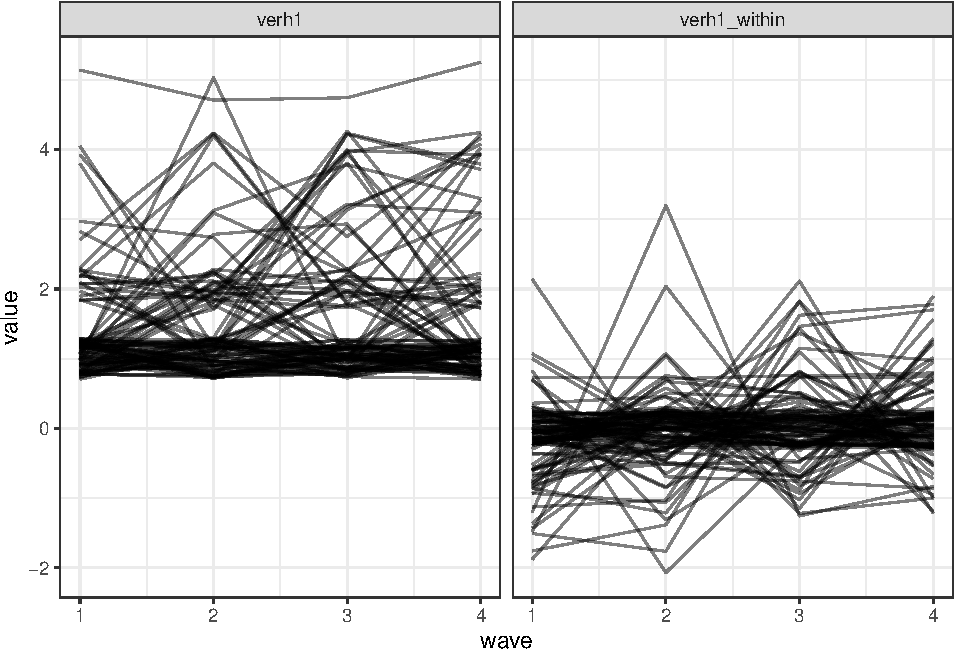
\includegraphics{workshop_panel_files/figure-latex/vis-ex2-1.pdf}

\begin{itemize}
\item
  Die Abbildung verdeutlicht dies anhand von 100 zufällig ausgewählten Personen aus dem Datensatz. Vor der Transformation gibt es (etwas) Varianz im Level des berichteten Verhaltens zwischen den Personen. Durch die Transformation verschwinden diese Unterschiede, es bleibt nur die Variation innhalb der Personen über die Zeit.
\item
  Das gleiche gilt für Prädiktoren, die als Merkmale anderer Einheiten, die wir als \emph{fixed effects} spezifiziert haben, konstant sind. In diesem Beispiel wären dies Eigenschaften der Perioden, also z.B. neue Schutzmaßnahmen bzw. deren Lockerung, soweit sie alle Personen gleichermaßen im gleichen Zeitraum betreffen.
\end{itemize}

\hypertarget{interaktionen-mit-personenmerkmalen}{%
\subsection*{Interaktionen mit Personenmerkmalen}\label{interaktionen-mit-personenmerkmalen}}
\addcontentsline{toc}{subsection}{Interaktionen mit Personenmerkmalen}

\begin{itemize}
\tightlist
\item
  Wir können jedoch Interaktionen zwischen über die Zeit variierenden Prädiktoren und Personenmerkmalen (oder Merkmalen anderer \emph{fixed effects} Einheiten) ins Modell aufnehmen.
\item
  Bei kategoriellen Moderator-Variablen erhalten wir Schätzer der Unterschiede zwischen gruppenspezifischen Effekten, z.B. den Unterschied zwischen den Effekten der Verhaltensintention auf das Verhalten für Frauen und Männer.
\item
  Bei kontinuierlichen Moderator-Variablen gelten die üblichen Fallstricke: Der Koeffizient des Prädiktors ist nun der einfache Effekt für den Fall, dass der Moderator gleich 0 ist. Der Koeffizient des Interaktionsterms quantifiziert den Unterschied des Effekts zwischen zwei Personen, die sich auf dem Moderator um eine Einheit unterscheiden.
\end{itemize}

\begin{Shaded}
\begin{Highlighting}[]
\NormalTok{d }\OperatorTok\StringTok{ }\KeywordTok{plm}\NormalTok{(verh1 }\OperatorTok{~}\StringTok{ }\NormalTok{verhint1 }\OperatorTok{*}\StringTok{ }\NormalTok{C_sex }\OperatorTok{+}\StringTok{ }\KeywordTok{factor}\NormalTok{(wave), }\DataTypeTok{data =}\NormalTok{ ., }\DataTypeTok{index =} \StringTok{"IDsosci"}\NormalTok{, }\DataTypeTok{model =} \StringTok{"within"}\NormalTok{) }\OperatorTok\StringTok{ }
\StringTok{    }\KeywordTok{tidy}\NormalTok{() }\OperatorTok\StringTok{ }\KeywordTok{mutate_if}\NormalTok{(is.numeric, round, }\DecValTok{2}\NormalTok{)}
\end{Highlighting}
\end{Shaded}

\begin{verbatim}
## # A tibble: 5 x 5
##   term           estimate std.error statistic p.value
##   <chr>             <dbl>     <dbl>     <dbl>   <dbl>
## 1 verhint1           0.34      0.03     13.2     0   
## 2 factor(wave)2      0.02      0.03      0.59    0.55
## 3 factor(wave)3      0.14      0.03      4.14    0   
## 4 factor(wave)4      0.12      0.03      3.42    0   
## 5 verhint1:C_sex    -0.01      0.03     -0.39    0.7
\end{verbatim}

\begin{itemize}
\tightlist
\item
  Der Effekt ist in der Stichprobe für Frauen minimal schwächer als für Männer. Der Unterschied ist jedoch weder substantiell noch statistisch bedeutsam.
\end{itemize}

\hypertarget{conclusio-vor--und-nachteile-des-fixed-effects-modells}{%
\section{\texorpdfstring{Conclusio: Vor- und Nachteile des \emph{fixed effects} Modells}{Conclusio: Vor- und Nachteile des fixed effects Modells}}\label{conclusio-vor--und-nachteile-des-fixed-effects-modells}}

\begin{quote}
In many applications the whole point of using panel data is to allow for \(a_i\) to be arbitrarily correlated with the \(x_{it}\). A fixed effects analysis achieves this purpose explicitly. --- \citet{wooldridge10}, S. 300
\end{quote}

\begin{quote}
By controlling out context, FE models effectively cut out much of what is going on --- goings-on that are usually of interest to the researcher, the reader and the policy maker. We contend that models that control out, rather than explicitly model, context and heterogeneity offer overly simplistic and impoverished results that can lead to misleading interpretations. --- \citet{bellExplainingFixedEffects2015}, S. 134
\end{quote}

\begin{itemize}
\item
  Das \emph{fixed effects} Modell ist nützlich, wenn wir einen kausalen Effekt, der sich innerhalb von Einheiten (Personen) abspielt, schätzen wollen.
\item
  Das \emph{fixed effects} Modell kann keine Merkmale der Einheiten (Personen) als Prädiktoren berücksichtigen, da die gesamten einheiten(personen)spezifischen Unterschiede bereits durch die \emph{fixed effects} erklärt werden.
\item
  Wir interessieren uns aber häufig (auch) für die Unterschiede zwischen Einheiten (Personen). Das \emph{fixed effects} Modell macht Antworten auf solche Fragen unmöglich.
\item
  Ein weiterer, damit unverbundener Nachteil des \emph{fixed effects} Modells ist die starke Anfälligkeit für Messfehler. Die Transformation verringert die wahre Varianz deutlich, während große Teile der Messfehlervarianz erhalten bleiben (sie sind nicht personenspezifisch).
\end{itemize}

\hypertarget{uxfcbungsaufgaben-2}{%
\section{Übungsaufgaben 2}\label{uxfcbungsaufgaben-2}}

\begin{enumerate}
\def\labelenumi{\arabic{enumi})}
\tightlist
\item
  Schätze den kausalen Effekt der Informationshäufigkeit aus öffentlich-rechtlichen TV-Programmen (\texttt{med2}) auf die Intention, weniger als 1.5m Abstand zu einer Person zu halten, die nicht im eigenen Haushalt lebt (\texttt{verhint3}). Berücksichtige dabei auch die Periodeneffekte der Panelwellen. Siehe dazu auch Übung 1.

  \begin{itemize}
  \tightlist
  \item
    Verwende jetzt \texttt{plm} für die Schätzung.
  \item
    Nimm zusätzlich die Information aus Zeitungen und Zeitschriften (\texttt{med1}) in das Modell auf.
  \item
    Prüfe, ob sich der Effekt der Information aus Zeitungen und Zeitschriften nach Geschlecht (\texttt{C\_sex}) unterscheidet.
  \end{itemize}
\item
  Spezifiziere, schätze und interpretiere ein eigenes \emph{fixed effects} Modell mit Daten aus dem Beispieldatensatz. Nutze dabei alle Techniken (unterschiedliche Spezifikation, Standardfehler, Moderation, mehrere Prädiktoren), die du ausprobieren und zu denen du ggf. Fragen stellen willst.
\end{enumerate}

\hypertarget{random-effects-modelle}{%
\chapter{\texorpdfstring{\emph{Random effects} Modelle}{Random effects Modelle}}\label{random-effects-modelle}}

\begin{itemize}
\tightlist
\item
  In diesem Abschnitt beschäftigen wir uns mit \emph{random effects} Modellen. Zuerst führen wir die Modellklasse ein. Dann betrachten wir kurz, wie die Modelle in der Tradition der Ökonometrie mit \texttt{plm} spezifiziert werden können, bevor wir zur allgemeineren Umsetzung mit dem Paket für Mehrebenen- bzw. \emph{mixed effects} Modelle \texttt{lme4} kommen.
\end{itemize}

\hypertarget{einfuxfchrung-random-effects-modelle-fuxfcr-paneldaten}{%
\section{Einführung: Random effects Modelle für Paneldaten}\label{einfuxfchrung-random-effects-modelle-fuxfcr-paneldaten}}

\hypertarget{modellspezifikation}{%
\subsection*{Modellspezifikation}\label{modellspezifikation}}
\addcontentsline{toc}{subsection}{Modellspezifikation}

\begin{itemize}
\item
  Anstatt für jede Einheit (Person) eine separate Konstante \(\alpha_i\) zu schätzen, können wir den ``soft constraint'' \citep[S. 257]{gelmanDataAnalysisUsing2006} setzen, dass die personenspezifischen Konstanten bzw. Residuen einer Verteilung folgen:

  \begin{itemize}
  \tightlist
  \item
    \(\alpha_{i} ∼ \mathcal{N}(\mu_{\alpha},\sigma^2_\alpha)\) mit \(i = 1,...,n\)
  \end{itemize}
\item
  Das \emph{random effects} Panel-Modell wird geschätzt als

  \begin{itemize}
  \tightlist
  \item
    \(y_{it}=x_{it}'\beta + z_i'\gamma + v_{it}\)
  \item
    \(v_{it} = \alpha_{i} + u_{it}\)
  \item
    mit \(y_{it}\) über Personen (\(i\)) und Zeit (\(t\)) variierendes Kriterium, \(x_{it}'\) über Personen und Zeit variierende Prädiktoren, \(\beta\) Koeffizienten der über Personen und Zeit variierenden Prädiktoren, \(z_i'\) über Personen variierende Prädiktoren, \(\gamma\) Koeffizienten der über Personen variierenden Prädiktoren, \(v_{it}\) gesamter Fehlerterm, \(\alpha_{i}\) personenspezifische Konstanten, \(u_{it}\) Residuen.
  \end{itemize}
\item
  Damit die Schätzer für \(\beta'\) unverzerrt sind, müssen zwei Annahmen erfüllt sein:

  \begin{enumerate}
  \def\labelenumi{\arabic{enumi}.}
  \tightlist
  \item
    Keine über die Zeit konstante Heterogenität, deren Ursache nicht im Modell ist
  \end{enumerate}

  \begin{itemize}
  \tightlist
  \item
    \({\displaystyle \operatorname {E} (\alpha _{i}|x_{it})=\operatorname {E} (\alpha _{i})=0}\)
  \end{itemize}

  \begin{enumerate}
  \def\labelenumi{\arabic{enumi}.}
  \setcounter{enumi}{1}
  \tightlist
  \item
    Keine über die Zeit variierende Heterogenität, deren Ursache nicht im Modell ist
  \end{enumerate}

  \begin{itemize}
  \tightlist
  \item
    \({\displaystyle \operatorname {E} (u_{it}|x_{it},\alpha _{i})=0,\quad t=1,...,T.}\)
  \end{itemize}
\end{itemize}

\hypertarget{vorteile-der-random-effects-modelle-fuxfcr-panel-daten}{%
\subsection*{\texorpdfstring{Vorteile der \emph{random effects} Modelle für Panel-Daten}{Vorteile der random effects Modelle für Panel-Daten}}\label{vorteile-der-random-effects-modelle-fuxfcr-panel-daten}}
\addcontentsline{toc}{subsection}{Vorteile der \emph{random effects} Modelle für Panel-Daten}

\begin{itemize}
\tightlist
\item
  Schätzer für über die Zeit konstante Prädiktoren und gleichzeitig Konstante für jede Person.
\item
  Schätzer von über die Zeit variierenden und über die Zeit konstanten Prädiktoren können verglichen werden.
\item
  Vorhersagen für neue Personen außerhab der Stichprobe können unter Einbeziehung aller Informationen und unter Berücksichtigung der gesamten Unsicherheit gemacht werden.
\item
  Die Annahme honogener Treatment-Effekte kann gelockert werden (mit dem within-between-Modell; siehe nächsten Abschnitt).
\end{itemize}

\hypertarget{sind-die-annahmen-des-random-effects-modell-fuxfcr-paneldaten-jemals-erfuxfcllt}{%
\subsection*{\texorpdfstring{Sind die Annahmen des \emph{random effects} Modell für Paneldaten jemals erfüllt?}{Sind die Annahmen des random effects Modell für Paneldaten jemals erfüllt?}}\label{sind-die-annahmen-des-random-effects-modell-fuxfcr-paneldaten-jemals-erfuxfcllt}}
\addcontentsline{toc}{subsection}{Sind die Annahmen des \emph{random effects} Modell für Paneldaten jemals erfüllt?}

\begin{quote}
The only difference between RE and FE lies in the assumption they make about the relationship between υ and the observed predictors: RE models assume that the observed predictors in the model are not correlated with \(v\) while FE models allow them to be correlated.
\end{quote}

\begin{quote}
A moment's reflection on what \(v\) represents-----all unmeasured time-constant factors about the respondent-----should lead anyone to realize that the RE assumption is heroic in social research, to say the least.
\end{quote}

\begin{quote}
The idea that the characteristics we don't (or can't) measure (like personality or genetic influences) are uncorrelated with the things we usually do measure (like income or church attendance) is implausible. --- \citet{vaiseyWhatYouCan2017}, S. 47
\end{quote}

\hypertarget{hausman-test}{%
\subsection*{Hausman-Test}\label{hausman-test}}
\addcontentsline{toc}{subsection}{Hausman-Test}

\begin{itemize}
\tightlist
\item
  Der Hausman-Test prüft, ob das \emph{random effects} Modell konsistent ist (\textasciitilde{} geschätzt werden darf).
\item
  Nach der traditionellen Sichtweise der Ökonometrie spricht das Verwerfen der \(H_0\) im Hausman-Test gegen das Schätzen eines \emph{random effects} Modells.
\item
  Da das \emph{random effecs} Modell in der Lage ist, Forschungsfragen zu beantworten, an denen das \emph{fixed effects} Modell per Definition scheitert, lässt sich die Wahl des \emph{random effects} Modells auch inhaltlich begründen --- ohne einen Hausman-Test durchzuführen.
\item
  Der Hausman-Test kann mit der Funktion \texttt{plm::phtest()} durchgeführt werden.
\end{itemize}

\begin{Shaded}
\begin{Highlighting}[]
\KeywordTok{phtest}\NormalTok{(verh1 }\OperatorTok{~}\StringTok{ }\NormalTok{verhint1, }\DataTypeTok{data =}\NormalTok{ d, }\DataTypeTok{index =} \StringTok{"IDsosci"}\NormalTok{)}
\end{Highlighting}
\end{Shaded}

\begin{verbatim}
## 
##  Hausman Test
## 
## data:  verh1 ~ verhint1
## chisq = 300.58, df = 1, p-value < 2.2e-16
## alternative hypothesis: one model is inconsistent
\end{verbatim}

\begin{itemize}
\tightlist
\item
  In diesem Beispiel spricht der Hausman-Test dagegen, ein \emph{random effects} Modell zu schätzen.
\end{itemize}

\hypertarget{random-effects-modelle-mit-plm}{%
\section{\texorpdfstring{Random effects Modelle mit \texttt{plm}}{Random effects Modelle mit plm}}\label{random-effects-modelle-mit-plm}}

\begin{itemize}
\tightlist
\item
  \emph{Random effects} Modelle für Paneldaten in der ökonometrischen Tradition lassen sich mit \texttt{plm} schätzen. Die Schätzung erfolgt auf Basis von Transformationen im Least-squares-Framework (ich habe keine Ahnung, wie das funktioniert). Ich selbst nutze diese Funktionalität in der Praxis nicht. Die Modellspezifikationen sind im Folgenden der Vollständigkeit halber kurz aufgeführt.
\end{itemize}

\begin{Shaded}
\begin{Highlighting}[]
\CommentTok{# Einfaches RE Modell}
\NormalTok{d }\OperatorTok\StringTok{ }\KeywordTok{plm}\NormalTok{(verh1 }\OperatorTok{~}\StringTok{ }\NormalTok{verhint1, }\DataTypeTok{data =}\NormalTok{ ., }\DataTypeTok{index =} \StringTok{"IDsosci"}\NormalTok{, }\DataTypeTok{model =} \StringTok{"random"}\NormalTok{) }\OperatorTok\StringTok{ }\KeywordTok{summary}\NormalTok{()}
\end{Highlighting}
\end{Shaded}

\begin{verbatim}
## Oneway (individual) effect Random Effect Model 
##    (Swamy-Arora's transformation)
## 
## Call:
## plm(formula = verh1 ~ verhint1, data = ., model = "random", index = "IDsosci")
## 
## Balanced Panel: n = 576, T = 4, N = 2304
## 
## Effects:
##                   var std.dev share
## idiosyncratic 0.32064 0.56625 0.812
## individual    0.07443 0.27283 0.188
## theta: 0.2799
## 
## Residuals:
##      Min.   1st Qu.    Median   3rd Qu.      Max. 
## -2.444787 -0.105500 -0.072748  0.038935  3.647334 
## 
## Coefficients:
##             Estimate Std. Error z-value  Pr(>|z|)    
## (Intercept)  0.56905    0.02764  20.587 < 2.2e-16 ***
## verhint1     0.53198    0.01195  44.517 < 2.2e-16 ***
## ---
## Signif. codes:  0 '***' 0.001 '**' 0.01 '*' 0.05 '.' 0.1 ' ' 1
## 
## Total Sum of Squares:    1531.9
## Residual Sum of Squares: 823.22
## R-Squared:      0.46262
## Adj. R-Squared: 0.46239
## Chisq: 1981.77 on 1 DF, p-value: < 2.22e-16
\end{verbatim}

\begin{Shaded}
\begin{Highlighting}[]
\CommentTok{# Mit zusätzlichem Faktor Welle}
\NormalTok{d }\OperatorTok\StringTok{ }\KeywordTok{plm}\NormalTok{(verh1 }\OperatorTok{~}\StringTok{ }\NormalTok{verhint1, }\DataTypeTok{data =}\NormalTok{ ., }\DataTypeTok{index =} \KeywordTok{c}\NormalTok{(}\StringTok{"IDsosci"}\NormalTok{, }\StringTok{"wave"}\NormalTok{), }\DataTypeTok{model =} \StringTok{"random"}\NormalTok{, }
    \DataTypeTok{effect =} \StringTok{"twoways"}\NormalTok{) }\OperatorTok\StringTok{ }\KeywordTok{summary}\NormalTok{()}
\end{Highlighting}
\end{Shaded}

\begin{verbatim}
## Twoways effects Random Effect Model 
##    (Swamy-Arora's transformation)
## 
## Call:
## plm(formula = verh1 ~ verhint1, data = ., effect = "twoways", 
##     model = "random", index = c("IDsosci", "wave"))
## 
## Balanced Panel: n = 576, T = 4, N = 2304
## 
## Effects:
##                    var  std.dev share
## idiosyncratic 0.316542 0.562621 0.802
## individual    0.075459 0.274699 0.191
## time          0.002634 0.051326 0.007
## theta: 0.2845 (id) 0.5845 (time) 0.2541 (total)
## 
## Residuals:
##      Min.   1st Qu.    Median   3rd Qu.      Max. 
## -2.479856 -0.114351 -0.069742  0.041790  3.672248 
## 
## Coefficients:
##             Estimate Std. Error z-value  Pr(>|z|)    
## (Intercept) 0.572357   0.038978  14.684 < 2.2e-16 ***
## verhint1    0.530146   0.012141  43.666 < 2.2e-16 ***
## ---
## Signif. codes:  0 '***' 0.001 '**' 0.01 '*' 0.05 '.' 0.1 ' ' 1
## 
## Total Sum of Squares:    1494.2
## Residual Sum of Squares: 817.26
## R-Squared:      0.45304
## Adj. R-Squared: 0.4528
## Chisq: 1906.68 on 1 DF, p-value: < 2.22e-16
\end{verbatim}

\begin{Shaded}
\begin{Highlighting}[]
\CommentTok{# Mit FE für Welle}
\NormalTok{d }\OperatorTok\StringTok{ }\KeywordTok{plm}\NormalTok{(verh1 }\OperatorTok{~}\StringTok{ }\NormalTok{verhint1 }\OperatorTok{+}\StringTok{ }\KeywordTok{factor}\NormalTok{(wave), }\DataTypeTok{data =}\NormalTok{ ., }\DataTypeTok{index =} \StringTok{"IDsosci"}\NormalTok{, }\DataTypeTok{model =} \StringTok{"random"}\NormalTok{) }\OperatorTok\StringTok{ }
\StringTok{    }\KeywordTok{summary}\NormalTok{()}
\end{Highlighting}
\end{Shaded}

\begin{verbatim}
## Oneway (individual) effect Random Effect Model 
##    (Swamy-Arora's transformation)
## 
## Call:
## plm(formula = verh1 ~ verhint1 + factor(wave), data = ., model = "random", 
##     index = "IDsosci")
## 
## Balanced Panel: n = 576, T = 4, N = 2304
## 
## Effects:
##                   var std.dev share
## idiosyncratic 0.31654 0.56262 0.808
## individual    0.07546 0.27470 0.192
## theta: 0.2845
## 
## Residuals:
##      Min.   1st Qu.    Median   3rd Qu.      Max. 
## -2.504920 -0.134512 -0.067223  0.050991  3.693574 
## 
## Coefficients:
##                 Estimate Std. Error z-value Pr(>|z|)    
## (Intercept)    0.5664150  0.0330635 17.1311  < 2e-16 ***
## verhint1       0.5300058  0.0121863 43.4918  < 2e-16 ***
## factor(wave)2 -0.0453317  0.0353413 -1.2827  0.19960    
## factor(wave)3  0.0672896  0.0353937  1.9012  0.05728 .  
## factor(wave)4  0.0028266  0.0358023  0.0789  0.93707    
## ---
## Signif. codes:  0 '***' 0.001 '**' 0.01 '*' 0.05 '.' 0.1 ' ' 1
## 
## Total Sum of Squares:    1521.3
## Residual Sum of Squares: 816.62
## R-Squared:      0.46322
## Adj. R-Squared: 0.46229
## Chisq: 1983.94 on 4 DF, p-value: < 2.22e-16
\end{verbatim}

\begin{Shaded}
\begin{Highlighting}[]
\CommentTok{# Mit Prädiktor auf Personenebene (funktioniert nicht in FE, siehe oben)}
\NormalTok{d }\OperatorTok\StringTok{ }\KeywordTok{plm}\NormalTok{(verh1 }\OperatorTok{~}\StringTok{ }\NormalTok{verhint1 }\OperatorTok{+}\StringTok{ }\NormalTok{C_sex, }\DataTypeTok{data =}\NormalTok{ ., }\DataTypeTok{index =} \KeywordTok{c}\NormalTok{(}\StringTok{"IDsosci"}\NormalTok{, }\StringTok{"wave"}\NormalTok{), }\DataTypeTok{model =} \StringTok{"random"}\NormalTok{, }
    \DataTypeTok{effect =} \StringTok{"twoways"}\NormalTok{) }\OperatorTok\StringTok{ }\KeywordTok{summary}\NormalTok{()}
\end{Highlighting}
\end{Shaded}

\begin{verbatim}
## Twoways effects Random Effect Model 
##    (Swamy-Arora's transformation)
## 
## Call:
## plm(formula = verh1 ~ verhint1 + C_sex, data = ., effect = "twoways", 
##     model = "random", index = c("IDsosci", "wave"))
## 
## Balanced Panel: n = 576, T = 4, N = 2304
## 
## Effects:
##                    var  std.dev share
## idiosyncratic 0.316542 0.562621 0.803
## individual    0.074785 0.273468 0.190
## time          0.002634 0.051326 0.007
## theta: 0.283 (id) 0.5845 (time) 0.2527 (total)
## 
## Residuals:
##      Min.   1st Qu.    Median   3rd Qu.      Max. 
## -2.443232 -0.153532 -0.048115  0.047936  3.701927 
## 
## Coefficients:
##              Estimate Std. Error z-value  Pr(>|z|)    
## (Intercept)  0.642039   0.045454 14.1249 < 2.2e-16 ***
## verhint1     0.527641   0.012153 43.4168 < 2.2e-16 ***
## C_sex       -0.106628   0.035587 -2.9963  0.002733 ** 
## ---
## Signif. codes:  0 '***' 0.001 '**' 0.01 '*' 0.05 '.' 0.1 ' ' 1
## 
## Total Sum of Squares:    1497.8
## Residual Sum of Squares: 815.06
## R-Squared:      0.45581
## Adj. R-Squared: 0.45534
## Chisq: 1927.32 on 2 DF, p-value: < 2.22e-16
\end{verbatim}

\hypertarget{kurze-einfuxfchrung-zu-mixed-effects-modellen}{%
\section{Kurze Einführung zu mixed effects Modellen}\label{kurze-einfuxfchrung-zu-mixed-effects-modellen}}

\begin{itemize}
\item
  Auch bekannt als \emph{random effects}, \emph{multilevel}/\emph{Mehrebenen-} oder \emph{hierarchical}/\emph{hierarchische} Modelle; das Begriffswirrwarr ist ein großes Problem, das Denglisch macht es nicht besser \citep{gelmanDataAnalysisUsing2006}.
\item
  Wer mit diesen Modellen bereits vertraut ist, kann diesen Absatz übersrpingen.
\item
  Ganz allgemein gesprochen sind \emph{mixed effects} Modelle Regressionsmodelle für Beobachtungen von Einheiten, die in irgendeiner Art miteinander zu tun haben, also nicht unabhängig voneinander sind.
\item
  Typische Beispiele sind Schüler*innen in Klassen in Schulen, Patient*innen in Krankenhäusern, Wähler*innen in Wahlkreisen, \ldots{} .
\item
  Paneldaten haben immer eine hierarchische Struktur: Beobachtungen (Level 1) sind innerhalb der Personen (Level 2) gruppiert.
\item
  Die Bezeichnung \emph{mixed effects} geht darauf zurück, dass in den Modellen sowohl \emph{random effects} (Koeffizienten, die zwischen den Fällen innerhalb einer Gruppierung auf einer höheren Ebene variieren) als auch \emph{fixed effects} (Koeffizienten, die für alle Fälle gleich sind) spezifiziert werden.
\end{itemize}

\hypertarget{warum-wir-in-den-sozialwissenschaften-nicht-nur-die-traditionellen-uxf6konometrischen-modelle-verwenden}{%
\subsection*{Warum wir in den Sozialwissenschaften nicht nur die traditionellen ökonometrischen Modelle verwenden}\label{warum-wir-in-den-sozialwissenschaften-nicht-nur-die-traditionellen-uxf6konometrischen-modelle-verwenden}}
\addcontentsline{toc}{subsection}{Warum wir in den Sozialwissenschaften nicht nur die traditionellen ökonometrischen Modelle verwenden}

\begin{quote}
Econometrics deal mostly with non-experimental data. Great emphasis is put on specification procedures and misspecification testing. Model specifications tend therefore to be very simple, while great attention is put on the issues of endogeneity of the regressors, dependence structures in the errors and robustness of the estimators under deviations from normality. --- \citet{plm2008}
\end{quote}

\begin{itemize}
\item
  Historische Gründe und disziplinäre Entwicklungen: z.B. Ökonometriker bevorzugen fast immer Least Squares, andere Disziplinen Maximum Likelihood oder Bayesianische Methoden.
\item
  Viele Sozialwissenschaften haben kompliziertere Datenstrukturen als das typische ökonometrische Panel, z.B. mehr als zwei Ebenen, nicht-hierarchische Datenstrukturen, heterogene Treatment-Effkte, \ldots{} . Die flexible Modellierung solcher Strukturen gilt oft als wichtiger als die enger gefassten Schätz- und Identifikationsfragen, die Ökonometriker umtreiben.
\item
  Die Ökonometrie betrachtet Abhängigkeitsstrukturen als eine Störgröße, deren Einfluss in den Modellen beschränkt werden soll. Andere sozialwissenschaftliche Disziplinen interessieren sich (auch, gerade) für diese Strukturen und ihre Konsequenzen.
\end{itemize}

\hypertarget{vorteile-der-mixed-effects-modelle}{%
\subsection{\texorpdfstring{Vorteile der \emph{mixed effects} Modelle}{Vorteile der mixed effects Modelle}}\label{vorteile-der-mixed-effects-modelle}}

\begin{itemize}
\item
  \emph{Mixed effects} Modelle bieten einen einheitlichen Rahmen für die Modellierung von Datensätzen mit jeder Art von Abhängigkeitstrukturen, seien sie hierarchisch, längsschnittlich oder eine Kombination aus beidem.
\item
  Die Schätzung basiert auf (Restricted) Maximum Likelihood, der Umstieg auf bayesianische Schätzmethoden ist relativ einfach. Im Vergleich dazu erfordern die Optionen, Tests und transformationsbasierten Least-Squares-Schätzer in der ökonometrischen Tradition erheblich mehr Einarbeitung, wenn man nicht auf eine entsprechende Ausbildung aufbauen kann.
\item
  Wenn man die Logik von \emph{mixed effects} Modellen einmal verstanden hat, kann man die Modelle für verschiedenste Forschungsfragen und -desings einsetzen, u.a. Ländervergleiche in der komparativen Forschung, experimentelle within-subject Desings, verschiedene Längsschnittsdesigns wie experience sampling, Tagebücher, digitale Kommunikations- und Verhaltensspuren, \ldots{} .
\item
  Das Denken in Varianzkomponenten (siehe nächster Absatz) hilft uns, konzeptionell über die Bedeutung von Prädiktoren auf verschiedenen Ebenen nachzudenken.
\item
  Einfache praktische Umsetzung: Das Paket \texttt{lme4} ist einfach zu verwenden, wenn man bereits etwas Erfahrung mit \texttt{stats::lm()} hat, und auch ein guter Einstieg in ähnlich aufgebaute Pakte zur bayesianischen Schätzung solcher Modelle (z.B. \texttt{rstanarm}, \texttt{brms}).
\end{itemize}

\hypertarget{varianzdekomposition-und-intraklassen-korrelation}{%
\subsection*{Varianzdekomposition und Intraklassen-Korrelation}\label{varianzdekomposition-und-intraklassen-korrelation}}
\addcontentsline{toc}{subsection}{Varianzdekomposition und Intraklassen-Korrelation}

\begin{itemize}
\item
  Wir interessieren uns dafür, welcher Anteil in der Varianz in \(Y\) auf stabile Unterschiede zwischen den Personen zurück geht und welcher auf Veränderungen innerhalb von Personen (potentielle kausale Effekte).
\item
  In \emph{mixed effects} Modellen können wir die Varianz-Anteile in einem sogenannten Null-Modell, das nur die Struktur der Daten abbildet, aber keine Prädiktoren enthält, bestimmen:

  \begin{itemize}
  \tightlist
  \item
    \(y_{it}= \alpha + v_{it}\) und \(v_{it} = \alpha_{i}+ u_{it}\)
  \end{itemize}
\item
  Ohne die Konstante \(\alpha\) erhalten wir

  \begin{itemize}
  \tightlist
  \item
    \(y_{it} = \alpha_{i}+ u_{it}\)
  \end{itemize}
\item
  Da die Varianzen von \(\alpha_i\) und \(u_{it}\) im Modell geschätzt werden, können wir den Anteil der personenspezifischen (Level 2) Varianz und den Anteil der idiosynkratischen Varianz in \(Y\) berechnen. Der Anteil der Level 2 Varianz an der gesamten Varianz wird auch als Intraklassen-Korrelation (intra-class correlation, ICC, \(\rho\)) bezeichnet.
\item
  In unserem Beispiel möchten wir wissen, welcher Anteil der Varianz im Verlassen der Wohnung ohne trifftigen Grund auf konstante Unterschiede zwischen den Personen zurückgeht (manche Personen wollen oder müssen, aus welchen Gründen auch immer, die Wohnung häufiger verlassen als andere).
\item
  Dazu spzifizieren wir das Null-Modell mit \texttt{lme4::lmer()}. Das genaue Vorgehen beim Spezifizieren der Modelle folgt im nächsten Abschnitt. Wichtig ist an dieser Stelle, dass mit \texttt{(1\ \textbar{}\ IDsosci)} jede Person eine eigene Konstante erhält (\(\alpha_i\) in der Gleichung oben), die als Abweichung vom Gesamtmittel (\(\alpha\)) geschätzt wird.
\end{itemize}

\begin{Shaded}
\begin{Highlighting}[]
\CommentTok{# Null-Modell}
\NormalTok{m0 =}\StringTok{ }\NormalTok{d }\OperatorTok\StringTok{ }\KeywordTok{lmer}\NormalTok{(verh1 }\OperatorTok{~}\StringTok{ }\DecValTok{1} \OperatorTok{+}\StringTok{ }\NormalTok{(}\DecValTok{1} \OperatorTok{|}\StringTok{ }\NormalTok{IDsosci), }\DataTypeTok{data =}\NormalTok{ .)}

\NormalTok{m0 }\OperatorTok\StringTok{ }\KeywordTok{summary}\NormalTok{()}
\end{Highlighting}
\end{Shaded}

\begin{verbatim}
## Linear mixed model fit by REML ['lmerMod']
## Formula: verh1 ~ 1 + (1 | IDsosci)
##    Data: .
## 
## REML criterion at convergence: 5576.4
## 
## Scaled residuals: 
##     Min      1Q  Median      3Q     Max 
## -4.1387 -0.2268 -0.1212 -0.1212  4.8131 
## 
## Random effects:
##  Groups   Name        Variance Std.Dev.
##  IDsosci  (Intercept) 0.5938   0.7706  
##  Residual             0.4065   0.6376  
## Number of obs: 2304, groups:  IDsosci, 576
## 
## Fixed effects:
##             Estimate Std. Error t value
## (Intercept)  1.52865    0.03475   43.99
\end{verbatim}

\begin{Shaded}
\begin{Highlighting}[]
\CommentTok{# ICC 'von Hand'}
\KeywordTok{round}\NormalTok{(}\FloatTok{0.5938}\OperatorTok{/}\NormalTok{(}\FloatTok{0.5938} \OperatorTok{+}\StringTok{ }\FloatTok{0.4065}\NormalTok{), }\DecValTok{3}\NormalTok{)}
\end{Highlighting}
\end{Shaded}

\begin{verbatim}
## [1] 0.594
\end{verbatim}

\begin{Shaded}
\begin{Highlighting}[]
\CommentTok{# Mit performance::icc()}
\KeywordTok{icc}\NormalTok{(m0)}
\end{Highlighting}
\end{Shaded}

\begin{verbatim}
## # Intraclass Correlation Coefficient
## 
##      Adjusted ICC: 0.594
##   Conditional ICC: 0.594
\end{verbatim}

\begin{Shaded}
\begin{Highlighting}[]
\CommentTok{# icc(lmer(verh1 ~ 1 + (1 | IDsosci) + (1 | wave), data = d), by_group = TRUE)}
\end{Highlighting}
\end{Shaded}

\begin{itemize}
\item
  Die Informationen zu den Varianzkomponenten findet sich im Output von \texttt{summary()} unter \texttt{Random\ effects}. Aus diesen Angaben können wir die ICC berechnen. Oder wir nutzen die Funktion \texttt{performance::icc()}.
\item
  Fast 60\% der Varianz im Verlassen der Wohnung geht auf Unterschiede zwischen Personen zurück.
\item
  Im \emph{fixed effects} Modell wird diese Varianz einfach aus den Daten entfernt. Über mehr als die Hälfte der Unterschiede können wir mit diesen Modellen also per Spezifikationslogik nichts aussagen.
\item
  Kausale Effekte innerhalb der Personen können damit \emph{maximal} für 40\% der Varianz verantwortlich sein.
\item
  Allerdings müssen wir dabei beachten, dass auch der gesamte Messfehler (zumindest die zufällige Messfehlervarianz nach der CTT) ebenfalls in diesem Varianzanteil steckt.
\item
  Wir können die Schätzer der \emph{random effects} für die Personen im Null-Modell auch dazu nutzen, uns einen Überblick zu verschaffen über die Verteilung der personenspezifischen Tendenz, die Wohnung ohne triftigen Grund zu verlassen. Die Schätzer können wir mit \texttt{ranef()} extrahieren, mit \texttt{broom.mixed::augment()} erhalten wir zusätzlich Standardfehler und Konfidenzintervalle in einem tidy data.frame.
\end{itemize}

\begin{Shaded}
\begin{Highlighting}[]
\CommentTok{# Verteilung der RE als Histogramm}
\NormalTok{m0 }\OperatorTok\StringTok{ }\KeywordTok{ranef}\NormalTok{() }\OperatorTok\StringTok{ }\KeywordTok{augment}\NormalTok{(}\DataTypeTok{ci.level =} \FloatTok{0.95}\NormalTok{) }\OperatorTok\StringTok{ }\KeywordTok{ggplot}\NormalTok{(}\KeywordTok{aes}\NormalTok{(estimate)) }\OperatorTok{+}\StringTok{ }\KeywordTok{geom_histogram}\NormalTok{()}
\end{Highlighting}
\end{Shaded}

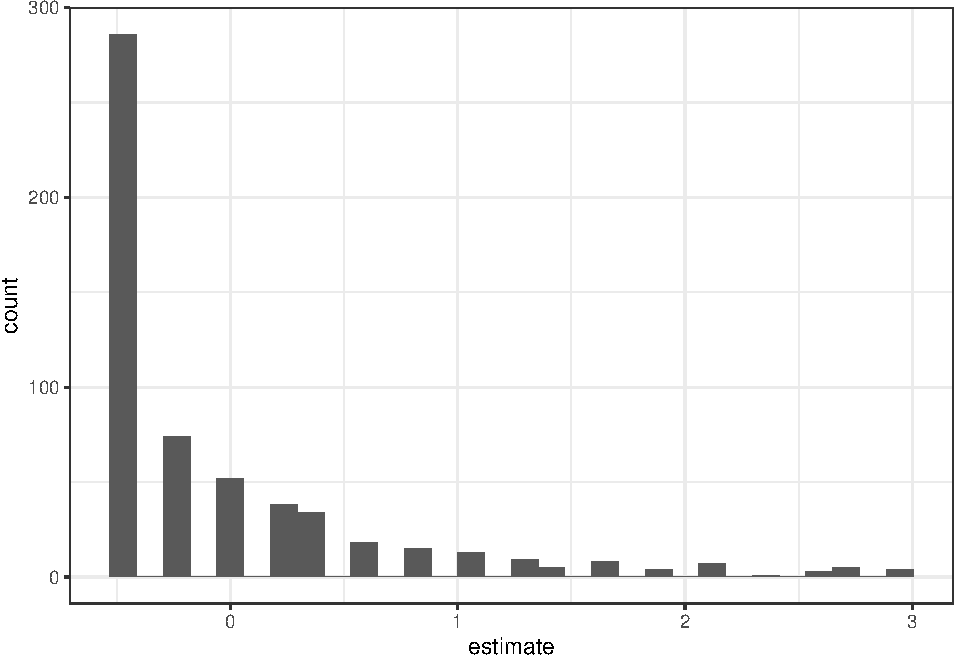
\includegraphics{workshop_panel_files/figure-latex/ranef-1.pdf}

\begin{Shaded}
\begin{Highlighting}[]
\CommentTok{# RE mit 95%-CIs (aus Darstellungsgründen nur jede fünfte Person)}
\NormalTok{m0 }\OperatorTok\StringTok{ }\KeywordTok{ranef}\NormalTok{() }\OperatorTok\StringTok{ }\KeywordTok{augment}\NormalTok{(}\DataTypeTok{ci.level =} \FloatTok{0.95}\NormalTok{) }\OperatorTok\StringTok{ }\KeywordTok{slice}\NormalTok{(}\KeywordTok{seq}\NormalTok{(}\DecValTok{1}\NormalTok{, }\KeywordTok{nrow}\NormalTok{(.), }\DataTypeTok{by =} \DecValTok{5}\NormalTok{)) }\OperatorTok\StringTok{ }
\StringTok{    }\KeywordTok{ggplot}\NormalTok{(}\KeywordTok{aes}\NormalTok{(estimate, level, }\DataTypeTok{xmin =}\NormalTok{ lb, }\DataTypeTok{xmax =}\NormalTok{ ub)) }\OperatorTok{+}\StringTok{ }\KeywordTok{geom_pointrangeh}\NormalTok{() }\OperatorTok{+}\StringTok{ }\KeywordTok{labs}\NormalTok{(}\DataTypeTok{y =} \StringTok{"IDsosci"}\NormalTok{)}
\end{Highlighting}
\end{Shaded}

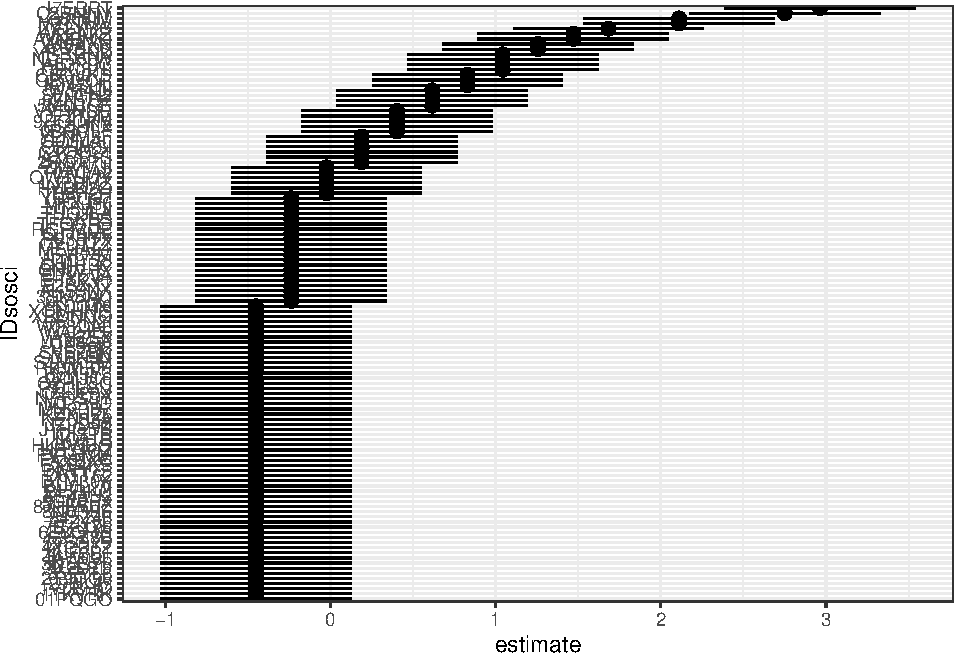
\includegraphics{workshop_panel_files/figure-latex/ranef-2.pdf}

\begin{itemize}
\tightlist
\item
  Der \emph{random effects} Schätzer quantifziert die Abweichung vom Schätzer der Konstanten in der Gesamtpopulation, hier die Abweichung von 1.5. Die diskreten Werte kommen zustande, da es (wie bei einer Index-Bildung) mit 5 Ausprägungen und 4 Wellen nur eine begrenzte Anzahl an möglichen Personen-Mittelwerten gibt.
\item
  Die Mehrheit der Personen tendiert dazu, eher selten ihre Wohnung ohne trifftigen Grund zu verlassen.
\end{itemize}

\hypertarget{mehr-als-ein-gruppierungsfaktor}{%
\subsection*{Mehr als ein Gruppierungsfaktor}\label{mehr-als-ein-gruppierungsfaktor}}
\addcontentsline{toc}{subsection}{Mehr als ein Gruppierungsfaktor}

\begin{itemize}
\tightlist
\item
  Mit \texttt{lme4} können prinzipiell beliebig viele und arbiträr angeordnete (sie müssen nicht hierarchisch sein) \emph{random effects} in ein Modell aufgenommen werden.
\item
  Zu viele Faktoren oder Faktoren mit zu wenigen Ausprägungen können aber zu Problemen bei der (restricted) maximum likelihood Schätzung führen (Bayesianische Schätzverfahren können hier helfen).
\item
  Wir könnten z.B. die geographische Region, in der die Personen leben, als einen weiteren, hierarchisch überhalb der Person angesiedelten Faktor aufnehmen. Hätten wir eine sehr große Stichprobe mit ausreichend geographischer Variation, wäre dies spannend, da wir uns durchaus regionale Unterschiede vorstellen könnten.
\item
  In Panel-Modellen liegt die Idee nahe, \emph{random effects} für die Panel-Wellen aufzunehmen. Dieser Faktor ist nicht hierarchisch zu den Personen. Stattdessen gehört jede Messung zu genau einer Person und genau einer Welle. Diese Spezifikation wird auch \emph{kreuzklassifiziert} / \emph{cross-classified} / \emph{crossed} genannt.

  \begin{itemize}
  \tightlist
  \item
    Wir nehmen den Faktor Welle auf, indem wir \texttt{+\ (1\ \textbar{}\ wave)} in der Modell-Formel ergänzen.
  \item
    Da wir nur Daten aus vier Wellen haben und die Varianz zwischen den Wellen sehr klein ist, kommt die \emph{restricted maximum likelihood} Schätzung hier an ihre Grenzen. Eine Warnung wird ausgegeben. Wir könnten das Problem durch Herumfrickeln an den Einstellungen des Optimizer beheben, würden aber inhaltlich zu keiner anderen Schlussfolgerungen kommen. Um den Einstieg in die technischen Details zu vermeiden, verwenden wir hier aber das Modell mit der Warnmeldung.
  \item
    Im Weiteren lösen wir das Problem, indem wir \emph{fixed effects} für die Wellen aufnehmen.
  \end{itemize}
\end{itemize}

\begin{Shaded}
\begin{Highlighting}[]
\CommentTok{# Null-Modell mit zwei Gruppierungsfaktoren}
\NormalTok{d }\OperatorTok\StringTok{ }\KeywordTok{lmer}\NormalTok{(verh1 }\OperatorTok{~}\StringTok{ }\DecValTok{1} \OperatorTok{+}\StringTok{ }\NormalTok{(}\DecValTok{1} \OperatorTok{|}\StringTok{ }\NormalTok{IDsosci) }\OperatorTok{+}\StringTok{ }\NormalTok{(}\DecValTok{1} \OperatorTok{|}\StringTok{ }\NormalTok{wave), }\DataTypeTok{data =}\NormalTok{ .) }\OperatorTok\StringTok{ }\KeywordTok{icc}\NormalTok{(}\DataTypeTok{by_group =} \OtherTok{TRUE}\NormalTok{)}
\end{Highlighting}
\end{Shaded}

\begin{verbatim}
## Warning in checkConv(attr(opt, "derivs"), opt$par, ctrl = control$checkConv, :
## Model failed to converge with max|grad| = 0.00262857 (tol = 0.002, component 1)
\end{verbatim}

\begin{verbatim}
## # ICC by Group
## 
## Group   |   ICC
## ---------------
## IDsosci | 0.595
## wave    | 0.018
\end{verbatim}

\begin{itemize}
\tightlist
\item
  Nur ein sehr geringer Teil der gesamten Varianz geht auf über alle Personen homogene Veränderungen zwischen den Wellen zurück.
\end{itemize}

\hypertarget{uxfcbungsaufgaben-3}{%
\section{Übungsaufgaben 3}\label{uxfcbungsaufgaben-3}}

\begin{enumerate}
\def\labelenumi{\arabic{enumi})}
\tightlist
\item
  Analysiere die Varianzkomponenten in der Intention, weniger als 1.5m Abstand zu einer Person zu halten, die nicht im eigenen Haushalt lebt (\texttt{verhint3}).

  \begin{itemize}
  \tightlist
  \item
    Spezifiziere zuerst ein Modell mit \emph{random effects} für die Personen.
  \item
    Nimm dann die Welle als zweiten Gruppierungsfaktor auf.
  \end{itemize}
\item
  Analysiere die Varianzkomponenten in weiteren Variablen, die dich interessieren.
\end{enumerate}

\hypertarget{within-between-models}{%
\chapter{Within-between models}\label{within-between-models}}

XXX

\bibliography{book.bib,packages.bib,references.bib}

\end{document}
